        %%******************************************%%
        %%                                          %%
        %%        Modello di tesi di laurea         %%
        %%            di Andrea Giraldin            %%
        %%                                          %%
        %%             2 novembre 2012              %%
        %%                                          %%
        %%******************************************%%

%**************************************************************
% file contenente le impostazioni della tesi
%**************************************************************


%**************************************************************
% Impostazioni di impaginazione
% see: http://wwwcdf.pd.infn.it/AppuntiLinux/a2547.htm
%**************************************************************

\setlength{\parindent}{14pt}   % larghezza rientro della prima riga
\setlength{\parskip}{0pt}   % distanza tra i paragrafi



%**************************************************************
% Impostazioni di biblatex
%**************************************************************
\bibliography{bibliografia} % database di biblatex 

\defbibheading{bibliography} {
    \cleardoublepage
    \phantomsection 
    \addcontentsline{toc}{chapter}{\bibname}
    \chapter*{\bibname\markboth{\bibname}{\bibname}}
}

\setlength\bibitemsep{1.5\itemsep} % spazio tra entry

\DeclareBibliographyCategory{opere}
\DeclareBibliographyCategory{web}

\addtocategory{opere}{womak:lean-thinking}
\addtocategory{web}{site:agile-manifesto}

\defbibheading{opere}{\section*{Riferimenti bibliografici}}
\defbibheading{web}{\section*{Siti Web consultati}}


%**************************************************************
% Impostazioni di caption
%**************************************************************
\captionsetup{
    tableposition=top,
    figureposition=bottom,
    font=small,
    format=hang,
    labelfont=bf
}

%**************************************************************
% Impostazioni di glossaries
%**************************************************************

%**************************************************************
% Acronimi
%**************************************************************
\renewcommand{\acronymname}{Acronimi e abbreviazioni}

%no acronimi e abbreviazioni

\iffalse
\newacronym[description={\glslink{apig}{Application Program Interface}}]
    {api}{API}{Application Program Interface}
\fi

%**************************************************************
% Glossario
%**************************************************************
%\renewcommand{\glossaryname}{Glossario}
\renewcommand{\glsnamefont}[1]{\makefirstuc{#1}}


%%%%%%%%%%%%%%%%%%%%%%%%%%%%%%%%%%%%%%%%%%%%%%%%%%%%%%%%%%%%%%%%%%%%%%%%%%%%

%no termini glossario
%tutto è definito subito in footnote

\iffalse
\newglossaryentry{asset}
{
    name=asset,
    sort=asset,
    description={todo}
}
\fi
 % database di termini
\makeglossaries


%**************************************************************
% Impostazioni di graphicx
%**************************************************************
\graphicspath{{immagini/}} % cartella dove sono riposte le immagini


%**************************************************************
% Impostazioni di hyperref
%**************************************************************
\hypersetup{
    %hyperfootnotes=false,
    %pdfpagelabels,
    %draft,	% = elimina tutti i link (utile per stampe in bianco e nero)
    colorlinks=true,
    linktocpage=true,
    pdfstartpage=1,
    pdfstartview=,
    % decommenta la riga seguente per avere link in nero (per esempio per la stampa in bianco e nero)
    %colorlinks=false, linktocpage=false, pdfborder={0 0 0}, pdfstartpage=1, pdfstartview=FitV,
    breaklinks=true,
    pdfpagemode=UseNone,
    pageanchor=true,
    pdfpagemode=UseOutlines,
    plainpages=false,
    bookmarksnumbered,
    bookmarksopen=true,
    bookmarksopenlevel=1,
    hypertexnames=true,
    pdfhighlight=/O,
    %nesting=true,
    %frenchlinks,
    urlcolor=webbrown,
    linkcolor=RoyalBlue,
    citecolor=webgreen,
    %pagecolor=RoyalBlue,
    %urlcolor=Black, linkcolor=Black, citecolor=Black, %pagecolor=Black,
    %pdftitle={\myTitle},
    %pdfauthor={\textcopyright\ \myName, \myUni, \myFaculty},
    %pdfsubject={},
    %pdfkeywords={},
    %pdfcreator={pdfLaTeX},
    %pdfproducer={LaTeX}
}

%**************************************************************
% Impostazioni di itemize
%**************************************************************
\renewcommand{\labelitemi}{$\bullet$}

%\renewcommand{\labelitemi}{$\bullet$}
%\renewcommand{\labelitemii}{$\cdot$}
%\renewcommand{\labelitemiii}{$\diamond$}
%\renewcommand{\labelitemiv}{$\ast$}


%**************************************************************
% Impostazioni di listings
%**************************************************************
\lstset{
    language=[LaTeX]Tex,%C++,
    keywordstyle=\color{RoyalBlue}, %\bfseries,
    basicstyle=\small\ttfamily,
    %identifierstyle=\color{NavyBlue},
    commentstyle=\color{Green}\ttfamily,
    stringstyle=\rmfamily,
    numbers=none, %left,%
    numberstyle=\scriptsize, %\tiny
    stepnumber=5,
    numbersep=8pt,
    showstringspaces=false,
    breaklines=true,
    frameround=ftff,
    frame=single
} 
\colorlet{punct}{red!60!black}
\definecolor{background}{HTML}{EEEEEE}
\definecolor{delim}{RGB}{20,105,176}
\colorlet{numb}{magenta!60!black}
\definecolor{codegreen}{rgb}{0,0.6,0}
\definecolor{codegray}{rgb}{0.5,0.5,0.5}
\definecolor{codepurple}{rgb}{0.82, 0.62, 0.91}
\definecolor{codeblue}{rgb}{0, 0.5, 1}
\definecolor{codeorange}{rgb}{1, 0.22, 0}

% Define the codebox
\lstdefinelanguage{dart}{
backgroundcolor=\color{background},   
    commentstyle=\color{codegreen},
    basicstyle=\ttfamily\footnotesize,
    breakatwhitespace=false,         
    breaklines=true, 
    stepnumber=1,
    captionpos=b,                    
    keepspaces=true,                 
    numbers=left,                    
    numbersep=8pt,                  
    showspaces=false,                
    showstringspaces=false,
    showtabs=false,                  
    tabsize=2,
    %frame=shadowbox
    emph=[1]{CheckLogin, HookWidget, Widget, BuildContext, bool, String, int, List, GenericErrorPage, LoginScreen, LoadUser, LoadCoach, DelayedWidget, Widget, Key, this, super, Future, false, true, Duration, Waiter, List, Goals, Appointment, ChangeNotifierProvider, UserRepo, Provider, ChangeNotifier, Reader, User, Options, Dio, Future },% Insert here the types you are using
    emphstyle=[1]{\color{codeblue}},
    emph=[2]{useProvider, build, useState, useEffect, delayed, then, buildCards, addAll, buildGoalsCards, where, map, toList, buildAppointmentCards, getAccessToken, fetchUser, watch, notifyListeners},% Insert here the methods you are using
    emphstyle=[2]{\color{codepurple}},
    emph=[3]{class, extends, @override, if, return, else, switch, case, default, final, required, is, as, =>, async, void, try, catch, finally, await},% Insert here the keywords you are using
    emphstyle=[3]{\color{codeorange}},%
}

\lstdefinelanguage{json}{
    basicstyle=\ttfamily\footnotesize,
    numbers=left,
    numberstyle=\scriptsize,
    stepnumber=1,
    numbersep=8pt,
    showstringspaces=false,
    breaklines=true,
    backgroundcolor=\color{background},
    string=[s]{"}{"},
    stringstyle=\color{blue},
    comment=[l]{:},
    commentstyle=\color{black},
    literate=
     *{0}{{{\color{numb}0}}}{1}
      {1}{{{\color{numb}1}}}{1}
      {2}{{{\color{numb}2}}}{1}
      {3}{{{\color{numb}3}}}{1}
      {4}{{{\color{numb}4}}}{1}
      {5}{{{\color{numb}5}}}{1}
      {6}{{{\color{numb}6}}}{1}
      {7}{{{\color{numb}7}}}{1}
      {8}{{{\color{numb}8}}}{1}
      {9}{{{\color{numb}9}}}{1}
      {:}{{{\color{punct}{:}}}}{1}
      {,}{{{\color{punct}{,}}}}{1}
      {[}{{{\color{delim}{[}}}}{1}
      {]}{{{\color{delim}{]}}}}{1},
}


%**************************************************************
% Impostazioni di xcolor
%**************************************************************
\definecolor{webgreen}{rgb}{0,.5,0}
\definecolor{webbrown}{rgb}{.6,0,0}


%**************************************************************
% Altro
%**************************************************************

\newcommand{\omissis}{[\dots\negthinspace]} % produce [...]

% eccezioni all'algoritmo di sillabazione
\hyphenation
{
    ma-cro-istru-zio-ne
    gi-ral-din
}

\newcommand{\sectionname}{sezione}
\addto\captionsitalian{\renewcommand{\figurename}{Figura}
                       \renewcommand{\tablename}{Tabella}}

\newcommand{\glsfirstoccur}{\ap{{[g]}}}

\newcommand{\intro}[1]{\emph{\textsf{#1}}}

%**************************************************************
% Environment per ``rischi''
%**************************************************************
\newcounter{riskcounter}                % define a counter
\setcounter{riskcounter}{0}             % set the counter to some initial value

%%%% Parameters
% #1: Title
\newenvironment{risk}[1]{
    \refstepcounter{riskcounter}        % increment counter
    \par \noindent                      % start new paragraph
    \textbf{\arabic{riskcounter}. #1}   % display the title before the 
                                        % content of the environment is displayed 
}{
    \par\medskip
}

\newcommand{\riskname}{Rischio}

\newcommand{\riskdescription}[1]{\textbf{\\Descrizione:} #1.}

\newcommand{\risksolution}[1]{\textbf{\\Soluzione:} #1.}

%**************************************************************
% Environment per ``use case''
%**************************************************************
\newcounter{usecasecounter}             % define a counter
\setcounter{usecasecounter}{0}          % set the counter to some initial value

%%%% Parameters
% #1: ID
% #2: Nome
\newenvironment{usecase}[2]{
    \renewcommand{\theusecasecounter}{\usecasename #1}  % this is where the display of 
                                                        % the counter is overwritten/modified
    \refstepcounter{usecasecounter}             % increment counter
    \vspace{10pt}
    \par \noindent                              % start new paragraph
    {\large \textbf{\usecasename #1: #2}}       % display the title before the 
                                                % content of the environment is displayed 
    \medskip
}{
    \medskip
}

\newcommand{\usecasename}{UC}

\newcommand{\usecaseactors}[1]{\textbf{\\Attori Principali:} #1. \vspace{4pt}}
\newcommand{\usecasepre}[1]{\textbf{\\Precondizioni:} #1. \vspace{4pt}}
\newcommand{\usecasedesc}[1]{\textbf{\\Descrizione:} #1. \vspace{4pt}}
\newcommand{\usecasepost}[1]{\textbf{\\Postcondizioni:} #1. \vspace{4pt}}
\newcommand{\usecasealt}[1]{\textbf{\\Scenario Alternativo:} #1. \vspace{4pt}}

%**************************************************************
% Environment per ``namespace description''
%**************************************************************

\newenvironment{namespacedesc}{
    \vspace{10pt}
    \par \noindent                              % start new paragraph
    \begin{description} 
}{
    \end{description}
    \medskip
}

\newcommand{\classdesc}[2]{\item[\textbf{#1:}] #2}
%**************************************************************
%cose mie
\definecolor{red}{cmyk}{0,0.87,0.68,0.32}
\newcolumntype{C}[1]{>{\centering\let\newline\\\arraybackslash\hspace{0pt}}m{#1}}

\newcommand{\vsc}{{Visual Studio Code}}
\newcommand{\astudio}{{Android Studio}}
%\newcommand{\flutter}{\textit{Flutter}} %nomi propri no corsivo
%\newcommand{\swift}{\textit{Swift}}
%\newcommand{\kotlin}{\textit{Kotlin}}
%\newcommand{\java}{\textit{Java}}
%\newcommand{\unity}{\textit{Unity}}
%\newcommand{\dart}{\textit{Dart}}
\newcommand{\arplug}{{ar\_flutter\_plugin}}
%\newcommand{\arcore}{\textit{ARCore}}
\newcommand{\aws}{Amazon Web Services}
\newcommand{\asa}{Azure Spatial Anchors}

\newcommand{\todo}{\textbf{\large{\textcolor{todoOrange}{TODO}}}}
%\newcommand{\E}{\`E} %maiuscole con apostrofo e non accento
\newcommand{\aCapo}{ ~ \vspace{0.22cm} \\} %magari fare renewcommand di paragraph 



\begin{document}
%\pagecolor{blond} %per occhi
%**************************************************************
% Materiale iniziale
%**************************************************************
\frontmatter
\input{inizio-fine/frontespizio}
\input{inizio-fine/colophon}
% !TEX encoding = UTF-8
% !TEX TS-program = pdflatex
% !TEX root = ../tesi.tex

%**************************************************************
% Sommario
%**************************************************************
\cleardoublepage
\phantomsection
\pdfbookmark{Sommario}{Sommario}
\begingroup
\let\clearpage\relax
\let\cleardoublepage\relax
\let\cleardoublepage\relax

\chapter*{Sommario}

Il presente documento è il resoconto della mia attività di tirocinio, della durata di circa trecentoventi ore, presso l'azienda Datasoil S.r.l.\\
L'obiettivo principale è stato la progettazione e l'implementazione di un'applicazione multipiattaforma legata al mondo del wellness/fitness a supporto della piattaforma di analisi dati realizzata per un prodotto spinoff dell'azienda. Il tutto con un focus sull'usabilità e l'engagement/gamification.\\
Il prodotto è stato sviluppato utilizzando Dart come linguaggio di programmazione e Flutter come framework. In questo modo è stato possibile scrivere un'unica applicazione che possa funzionare sia su dispositivi Android, sia su dispositivi iOS.

%\vfill
%
%\selectlanguage{english}
%\pdfbookmark{Abstract}{Abstract}
%\chapter*{Abstract}
%
%\selectlanguage{italian}

\endgroup			

\vfill


% !TEX encoding = UTF-8
% !TEX TS-program = pdflatex
% !TEX root = ../tesi.tex

%**************************************************************
% Ringraziamenti
%**************************************************************
\cleardoublepage
\phantomsection
\pdfbookmark{Ringraziamenti}{ringraziamenti}

\bigskip

\begingroup
\let\clearpage\relax
\let\cleardoublepage\relax
\let\cleardoublepage\relax

\chapter*{Ringraziamenti}

\noindent \textit{Innanzitutto, vorrei esprimere la mia gratitudine al Prof. Tullio Vardanega, relatore della mia tesi, per il supporto preciso e puntuale fornitomi durante l'intera durata dello stage e la conseguente stesura della tesi.}\\

\noindent \textit{Un ringraziamento va ad Andrea e Pietro, riferimenti aziendali, e in generale a tutto il team Datasoil S.r.l. che mi ha permesso di vivere un'esperienza arricchente in un ambiente lavorativo sereno.}\\

\noindent \textit{Desidero infine ringraziare i miei familiari senza i quali mai avrei potuto intraprendere un percorso impegnativo come un corso di laurea.}\\


\bigskip

\noindent\textit{\myLocation, \myTime}
\hfill \myName

\endgroup


\input{inizio-fine/indici}
\cleardoublepage

%**************************************************************
% Materiale principale
%**************************************************************
\mainmatter
% !TEX encoding = UTF-8
% !TEX TS-program = pdflatex
% !TEX root = ../tesi.tex

%**************************************************************
\chapter{Contesto Aziendale}
\label{cap:contesto-aziendale}
%**************************************************************

\section{L'azienda}
\subsection{Descrizione}
Le informazioni a seguito sono state prese direttamente dall'azienda, tuttavia ritengono siano rappresentative della realtà considerando sia il progetto al quale ho partecipato, sia il resto dell'offerta \textit{software}.\\
\textbf{Datasoil S.r.l.} è una \textit{startup} innovativa che si occupa di sviluppare applicativi dedicati alla gestione aziendale, altamente integrati con industria 4.0 e \textit{digital twin}: vengono impiegati \textit{machine learning} e analisi predittive per ottenere analitiche migliori rispetto alla concorrenza, con un occhio attento a innovazione, sicurezza e scalabilità, ottenute tramite prototipazione e \textit{Infrastrucutre as Code}, delegando quindi la gestione delle componenti \textit{server} a servizi terzi come \aws{} (ecosistema \textit{software} fornito da Amazon, che va da semplici piattaforme di \textit{cloud storage} fino a sistemi predittivi basati su \textit{machine learning}).\\
Il loro obiettivo è manipolare ed elaborare dati di natura inerentemente caotica, ordinarli e presentarli all'utente finale tramite interfacce grafiche intuitive, promuovendo un'interazione efficace tra utilizzatore e mezzo. Prediligono un approccio ai problemi condiviso e modulare per far nascere soluzioni inedite da applicare a grandi progetti, forti di un \textit{know-how} che abbraccia esigenze verticali (vengono impiegate internamente molte tecnologie sia lato \textit{frontend} che lato \textit{backend}).\\
Le piattaforme dedicate ad \textit{industry} 4.0, \textit{smart building} e \textit{smart city} poggiano su dei \textit{data silos} attualmente esistenti, garantendo un'interpretazione integrata e di alto livello delle informazioni aziendali fondendole con eventi provenienti dai diversi \textit{business level} creando \textit{insight} proattivi in tempo reale. I sistemi predittivi di Datasoil sono in grado di notificare la persona giusta al momento giusto anticipando la gestione delle criticità interfunzionali.\\
Ho avuto modo di verificare molte di queste affermazioni direttamente tramite il progetto proposto, in quanto si tratta di un applicativo legato all'industria 4.0 che mappa \textit{asset} aziendali (come ad esempio macchinari) ad un gemello digitale, permettendo sia di localizzarli su una mappa tridimensionale sia, obiettivo dello stage, di visualizzarli in realtà aumentata.\\

\subsection{Clientela}
Datasoil sviluppa applicazioni che guardano al mondo professionale più che a quello generico \textit{consumer}, ad esempio in questo specifico caso l'applicativo (che prende il nome di MobileSYN) è dedicato a un'utenza strettamente aziendale, e ci si aspetta che venga utilizzata da operatori interni con dispositivi controllati (generalmente \textit{tablet} Apple). \\
Anche un altro prodotto dell'azienda, chiamato LifestyleSync, mira a fornire uno strumento per migliorare il benessere dei dipendenti nelle aziende, permettendo a ogni dipendente di essere seguito da un \textit{coach} che, tramite un'applicazione di supporto LSCoach, può progettare allenamenti personalizzati e vedere la progressione degli stessi.

\subsection{Processi Interni}

\subsection{Innovazione}
%************************************************************************************************************
\section{Tecnologie e Strumenti}
\label{sec:tecnologie-e-strumenti}

\subsection{Tecnologie e Strumenti di sviluppo}
\subsubsection{Visual Studio Code}
\vsc{} è un editor per codice sorgente, sviluppato da \textit{Microsoft} servendosi del framework \textit{Electron}, disponibile per Windows, Linux e macOS. Le sue funzionalità comprendo supporto per debugging, syntax highlighting, intelligent code completion, snippets, code refactoring, e integrazione con Git. \\
Gli utenti possono configurare tema, macro, preferenze e installare estensioni che ne aumentano le funzionalità aggiungendo ad esempio il supporto ai maggiori linguaggi di porgrammazione attualmente presenti.\\
Nella \textit{Stack Overflow 2021 Developer Survey}, \vsc{} è risultato essere l'IDE più popolare, adottato dal 70\% degli intervistati. {\tiny Fonte: \href{https://en.wikipedia.org/wiki/Visual_Studio_Code}{Wikipedia}}\\
\E{} inoltre presente e molto comoda l'estensione di \flutter{} che, tra le altre cose, permette di gestire direttamente in gui i vari dispositivi (smartphone, browser o emulatore) sui quali installare e lanciare l'app che si sta programmando.

\subsubsection{Android Studio}
\textit{Android Studio} è l'IDE ufficiale del sistema operativo di Gooogle, sostituendo Eclipse dal 2015, costruito sul software IntelliJ di JetBrains e progettato specificatamente per lo sviluppo Android. \E{} disponibile per Windows, Linux e macOS.\\
Il 7 maggio 2019 Kotlin rimpiazzò Java come linguaggio consigliato per Android, favorendo un'integrazione ancora maggiore con JetBrains che, appunto, ha sviluppato e prodotto Kotlin stesso. {\tiny Fonte: \href{https://en.wikipedia.org/wiki/Android_Studio}{Wikipedia}}\\
Personalmente ho cercato nonostante tutto di programmare il più possibile su \vsc{} preferendolo quindi ad \textit{Android Studio} in virtù della sua maggiore leggerezza e delle sue più ampie possibilità di personalizzazione.

\subsubsection{Dart}
Dart è un linguaggio di programmazione sviluppato da Google per il client development, ovvero per web e mobile app, e può anche essere impiegato per la costruzione di applicazione desktop e server.\\
\E{} un linguaggio object-oriented, class-based, garbage-collected, strongly-typed e con una sintassi nello stile di C. Può compilare sia codice macchina che JavaScript e supporta interefacce, mixins, classi astratte, refined generics e type inference.{\tiny Fonte: \href{https://en.wikipedia.org/wiki/Dart_(programming_language)}{Wikipedia}}\\
Personalmente l'ho trovato elegante e conciso nella sua struttura, e presenta dei vantaggi consistenti come la null protection e le espressioni ternarie.

\subsubsection{Flutter}
Flutter è un framework open-source creato da Google per lo sviluppo della UI di applicazioni cross-platform per Android, iOS, Linux, macOS, Windows, Google Fuchsia e il web partendo da un singolo codebase.\\
Rialsciato a maggio 2017, le applicazioni in Flutter sono scritte in Dart e sfruttano molte delle features avanzate del linguaggio, e le componenti principali del framework sono:
\begin{itemize}
    \item \textbf{Dart platform:} Flutter gira all'interno della Dart Virtual Machine, che si serve di un execution engine just-in-time;
    \item \textbf{Flutter engine:} scritto primariamente in C++, fornisce supporto a basso livello per il rendering e implementa accessibilità, file e network I/O, supporto nativo per i plugin e molto altro;
    \item \textbf{Foundation library:} scritta in Dart, fornisce classi e funzioni di base che vengono usate per costruire gli applcativi in Flutter, come ad esempio le API per la comunicazione con l'engine;
    \item \textbf{Design-specific widgets:} Flutter contiene due famiglie di widget che si conformano a delle specifiche scuole di design: \textit{Material} per Google e \textit{Cupertino} per Apple;
    \item \textbf{Flutter DevTools:} famiglia di tools generici che vengono sfruttati per lo sviluppo di software in Flutter.
\end{itemize}
~\\
Inoltre, una libreria fondamentale per semplificare l'utilizzo di Flutter è \textit{Flutter Hooks}: lo scopo è implementare delle strutture simili agli Hooks di React, consentono di sostituire gli Stateful Widget riducendo il boilerplate code e semplificando la gestione di side-effect e ciclo di vita dei widget grazie alla funzione \textit{useEffect}.

\subsubsection{Java}
Java è un linguaggio di programmazione ad alto livello object-oriented progettato per avere il minor numero possibile di dipendenze implementative (favorendo quindi l'uso di interfacce e classi astratte) e, soprattutto, per aderire al motto \textit{"write once, run anywhere"}: il bytecode di Java può infatti girare senza necessità di ricompilazione su qualsiasi piattaforma che supporti la Java Virtual Machine (comunemente abbreviata in JVM).\\  
La sintassi è simile a quelle di C o C++, ma fornisce funzionalità dinamiche generalmente inedite per i linguaggi compilati, come reflection e modifica del codice a runtime.\\
Originalmente rilasciato nel 1995 come componente centrale della piattaforma Java per Sun Microsystems e sotto licenza proprietaria, dal 2007 la maggior parte dei suoi componenti sono diventati open-source sotto l'ombrello della \textit{GPL-2.0-only} (licenza specifica per software libero pubblicata dalla Free Software Foundation).\\
Sebbene Oracle (attuale proprietario di Sun Microsystems) offra un'implementazione proprietaria chiamata \textit{HotSpot JVM}, la specifica ufficiale è la \textit{OpenJDK JVM} che è gratuita, open-source e di default nella maggior parte delle distribuzioni Linux.

\subsubsection{Kotlin}
Kotlin è un linguaggio di programmazione cross-platform, staticamente tipizzato, progettato per avere completa interoperabilità con Java, gode di una sintassi più concisa di quest'ultimo grazie alla type inference di cui è dotato e dipende dalla \textit{Java Class Library} per la versione della JVM da usare.\\
\E{} inoltre in grado di compilare codice in JavaScript (sfruttato poi da applicazioni frontend) o codice nativo tramite \textit{LLVM} (per app iOS che condividono la business logic con applicazioni Android).\\
Incluso in Android Studio come alternativa al compilatore standard Java dal 2017, produce bytecode Java 8 di default ma permette al programmatore di scegliere delle versioni target successive (fino a Java 18).

\subsubsection{Azure Spatial Anchors}
Azure Spatial Anchors è un servizio di Microsoft mirato a fornire strumenti per sviluppare applicazioni in realtà aumentata su dispositivi iOS o Android predisposti per, rispettivamente, ARKit e ARCore, oppure su Microsoft HoloLens.\\
Permette di riconoscere spazi tridimensionali all'interno dei quali posizionare punti di interesse, chiamati Spatial Anchors, che possono essere salvati in cloud e poi recuperati, e possono essere messi in relazione a oggetti reali (come macchinari in un contesto industriale) o virtuali.

\subsubsection{ARCore}
ARCore, conosciuto anche come Google Play Services per AR, è un software development kit prodotto da Google per permettere lo sviluppo di applicazioni in realtà aumentata.\\
Si serve di tre componenti principali:
\begin{itemize}
    \item \textbf{6DOF:} il dispositivo sfrutta una piattaforma inerziale a sei assi per comprendere e tracciare la propria posizione relativa allo spazio;
    \item \textbf{Environmental understanding:} permette riconoscere dimensioni e locazione delle superfici lisce;
    \item \textbf{Light estimation:} permette al telefono di stimare le condizioni di luce dell'ambiente.
\end{itemize}
asa si appoggia proprio ad ARCore per implementare le proprie funzionalità di AR su Android.

\todo
\textcolor{todoOrange}{ar flutter plugin, sceneform?}


%**************************************************************
\subsection{Strumenti organizzativi}

\subsubsection{Slack}
Slack è una piattaforma di comunicazione istantanea di proprietà di Salesforce e sviluppata da Slack Technologies per Windows, Linux, macOS, Android e iOS.\\
Permette di comunicare tramite messaggi, chiamate vocali e video, e di inviare media e files nelle chat private o nei canali. Quest'ultimi fungono da aggregatori e permettono di suddividere tematicamente la comunicazione.\\
\E{} inoltre possibile suddividere a un livello ancora più alto tramite i \textit{workspaces}, che aggregano al proprio interno utenti, canali e applicazioni: sono proprio quest'ultime che mostrano con maggiore chiarezza l'orientamento \textit{corporate} di Slack, infatti fornisce integrazione nativa con i maggiori software gestionali e organizzativi (come ad esempio Jira, Zoom, Drive, Outlook, etc).

\subsubsection{Github}
GitHub è il più grande servizio di hosting di codice sorgente al mondo, abitualmente usato per sviluppare progetti open source, e fornisce vari servizi: version control di Git distribuito e access control, bug tracking, issue tracking, richieste di modifiche software, task management, integrazione continua e wiki per ogni progetto.\\ 
Permette inoltre, tramite forking, pull request e commenti, il miglioramento collaborativo del software, ad esempio risolvendo bug, aggiungendo funzionalità o migliorando quelle presenti.


% !TEX encoding = UTF-8
% !TEX TS-program = pdflatex
% !TEX root = ../tesi.tex

%**************************************************************
\chapter{Lo Stage}
\label{cap:lo-stage}
%**************************************************************
\section{Descrizione e temi}
Il progetto proposto prevede l'implementazione di una vista in realtà aumentata\footnote{Schermata che mostra il \textit{feed} della fotocamera e permette di interagirci come fosse uno spazio 3D renderizzato} per l'applicazione di ticketing e monitoraggio aziendale "\textbf{MobileSYN}".\\
Questo applicativo permette di creare un gemello digitale di un asset aziendale e posizionarlo all'interno di uno spazio virtuale tridimensionale, così da rendere visivamente più chiaro quali macchinari di un dato stabilimento industriale abbiano necessità di manutenzione (mediante apertura di ticket appositi).\\
Un ticket è semplicemente una notifica relativa ad un asset (perdita d'olio per un macchinario, carta esaurita per una stampante, etc) ma può anche essere libero da questo vincolo e trovarsi, in autonomia, posizionato nello spazio (ad esempio per segnalare una crepa su un muro).

\begin{figure}[ht]
    \centering
    \includegraphics[height=5cm]{plant_asset_screenshot}
    \caption{Asset "Compressor Intake" in stabilimento "Plant 1"}
\end{figure}

Tutte le funzionalità in realtà aumentata dovranno necessariamente appoggiarsi al servizio di \asa{} perchè i gemelli digitali già presenti nel sistema sfruttano proprio questa tecnologia per la propria localizzazione spaziale e, vista la natura multipiattaforma dell'applicazione, dovranno essere implementate sia in Android che in iOS.
Dalla vista dovrà essere possibile interagire con gli \textit{asset} e i \textit{ticket}, (posizionamento ed eliminazione in \textit{augmented reality}) provocando l'apparizione di una \textit{card} all' \textit{on-tap} dell'\textit{anchor}\footnote{Traducibile in italiano con il termine "angoraggio" è un punto di interesse in uno spazio tridimensionale, ovvero un punto che possiede delle coordinate \textit{(x,y,z)}, al quale possono essere collegati \textit{asset}, \textit{ticket} o altri ancoraggi.}, ovvero mostrando a schermo tramite una piccola finestra in sovraimpressione i vari ticket relativi all'\textit{asset} dopo che questo viene toccato, permettendo anche la visione del dettaglio o la rimozione dello stesso.

\begin{figure}[ht]
    \centering
    \includegraphics[height=5cm]{asset_card}
    \caption{\textit{Card} (in primo piano) relativa a una \textit{anchor} (in secondo piano) in vista in realtà aumentata}
\end{figure}

Per portare a termine gli obiettivi prefissati sarà necessario studiare dei \textit{framework}, dei \textit{plugin} o dei \sdk{} che permettono l'integrazione del codice nativo di \asa{} (che sarà Java per Android e Swift per iOS) con il \textit{framework} Flutter e il linguaggio su cui si poggia, ovvero Dart. 

\section{Strategia aziendale}
Da un punto di vista strettamente aziendale questo \textit{stage} è stato inquadrato in una strategia che prevede l'espansione di funzionalità per applicativi esistenti nell'ottica di fornire valore aggiunto ai clienti attuali e futuri: precedentemente a questo progetto non era presente alcuna componente in realtà aumentata in MobileSYN, mentre la strategia futura è un continuo miglioramento di ciò che è stato aggiunto. Infatti non sono state sufficienti otto settimane per ottenre un risultato professionalmente soddisfacente, e Datasoil nel futuro si occuperà di limare l'interfaccia grafica (anche osservando sul campo le abitudini d'uso della stessa da parte degli operatori) e migliorare pulizia ed efficienza del codice prodotto.\\
L'azienda si rapporta con gli \textit{stage} in un'ottica produttiva: si tratta spesso di attività che si innestano in lavori già in atto o che sarebbero comunqui stati eseguiti, tuttavia nel mio caso questo si è legato fortemente al concetto di innnovazione per la natura stessa del progetto che tratta, come già discusso, tematiche non comuni (nello specifico la realtà aumentata). L'azienda inoltre sfrutta gli \textit{stage} per effettuare un primo \textit{screening} per eventuali collaboratori da assumere.\\
L'azienda si è attivamente impiegata a supportare il mio \textit{stage} con tuttua una serie di attività: sono stato direttamente ospitato in azienda e ho avuto accesso a risorse aziendali (\textit{account} \aws{} per accedere a MobileSYN) e credenziali \asa{}, inoltre sia il \textit{junior} che il \textit{senior developer} di Datasoil che si occupano del lato \textit{frontend} mi hanno attivamente affiancato durante lo sviluppo nella fase di codifica. Ho inoltre ricevuto supporto nella fase di analisi dei requisiti e in altri piccoli problemi relativi alla configurazione dei dispositivi e dei programmi necessari ad affrontare lo \textit{stage}.

\section{Obiettivi}
\begin{itemize}
    \item Minimi:
        \begin{itemize}
            \item Studio e comprensione del linguaggio di programmazione Dart e del \textit{framework} Flutter;
            \item Analisi strumenti Azure: Azure Console e \asa{};
            \item Ricerca di \textit{framework} e \sdk{} per implementare le \asa{} in Flutter;
            \item Eventuale studio di linguaggi necessari alle implementazioni native, come ad esempio Kotlin, Java, Unity o Swift;
            \item Completamento del \textit{framework} scelto nell'app Flutter esistente;
            \item Completamento dello sviluppo dei componenti per rappresentare le \textit{anchor} nello spazio in realtà aumentata;
            \item Completamento dello sviluppo delle \api{} per l'interazione utente con gli ancoraggi in realtà aumentata;
        \end{itemize}
    \item Massimi: 
        \begin{itemize}
            \item Sviluppo di componenti per mappare \textit{asset} aziendali ad \textit{anchor};
            \item Sviluppo di componenti grafici per la visualizzazione di metriche e informazioni di controllo.
        \end{itemize}
\end{itemize}

\section{Vincoli}
Come precedentemente accennato, i vincoli in questo progetto sono due: 
\begin{itemize}
    \item Utilizzare Flutter come \textit{framework} sul quale implementare le componenti in realtà aumentata;
    \item La tecnologia scelta per gestire gli ancoraggi in realtà aumentata deve essere \asa{}.
\end{itemize}
Eccezion fatta per queste specifiche tecnologiche il resto è stato lasciato a mia discrezione personale, sebbene siano stati consigliati degli strumenti di sviluppo (\vsc{} e \astudio{} come \ide{}). 
Vincoli non tecnologici ma organizzativi sono da identificare nell'uso di Slack di GitHub: il primo usato per la comnicazione interna con i membri di dell'azienda, il secondo invece è il \textit{repository}\footnote{Spesso abbreviato con \textit{"repo"} è un generico archivio di codice sorgente e pacchetti \textit{software}. Spesso contiene anche \textit{metadata} e guide per la configurazione, uso ed estensione del codice che contiene. In genere un \textit{repo} ha una qualche forma di controllo di versione integrato.} dove si trova il codice sorgente di MobileSYN.

\section{Motivazione scelta}
I motivi che mi hanno spinto ad accettare questo stage rispetto ad altri sono molteplici, ma i principali sono quattro: toccare con mano attività legate al \textit{frontend}, vivere in prima persona l'ambiente di lavoro del mio ambito di studi, avere la possibilità di sviluppare in ambito \textit{mobile} e una personale curiosità nei confronti delle tecnologie trattate, ovvero la realtà aumentata.
Elaboro ora con più completezza i quattro punti di cui sopra: per quanto riguarda il \textit{frontend}, è un ambito o comunque sia una branca del mondo dello sviluppo \textit{software} che guardavo con interesse in quanto raramente ho avuto occasione di occuparmene durante il corso di studui. Infatti nella maggioranza dei progetti e degli \textit{assignment} trattati mi sono sempre occupato del lato \textit{backend}, infatti il cambio di approccio si è dimostrato difficoltoso, costringendomi a ragionare e a vedere il codice in maniera diversa. Flutter inoltre ha reso il tutto ancora più arduo siccome mischia aspetti di interfaccia grafica con logiche di controllo.\\
Vivere uno stage a contatto con degli sviluppatori di grado \textit{senior} e lavorare in un ambiente con un certo grado di controllo era per me molto importante: da una parte per garantirmi di assorbire conoscenze da personale esperto, dall'altra per assicurarmi di mantenere un \textit{focus} quanto più alto possibile durante il corso del progetto. Era inoltre fondamentale avere un'idea più chiara di come sia il mondo del lavoro in ambito \textit{software}.\\
Il terzo punto nasce da una considerazione: il mondo dello sviluppo \textit{mobile} è quello più ampio e in continua crescita. Ormai i \textit{computer} sono sempre più rari e vengno generalmente acquistati da persone ad alto livello di specializzazione, mentre il pubblico generalista preferisce acquistare \textit{smartphone} e \textit{tablet}. E' quindi saggio a mio avviso sviluppare delle competenze in questo ambito perchè saranno sicuramente molto spendibili.\\
Infine, il quarto ed ultimo motivo che mi ha spinto a scegliere questo \textit{stage} rispetto ad altri riguarda la tecnologia affrontata: trovo affascinante l'impiego della realtà aumentata perchè è molto poco comune e, probabilmente, diventerà man mano più diffusa con il passare degli anni. Inoltre tra quelle disponibili ho trovato intelligente da parte di Datasoil scegliere proprio quella di Microsoft che, forte di disponibilità economiche fuori misura, difficilmente abbandonerà un progetto sul quale ha già investito così largamente.\\
Naturalmente oltre a tutto ciò sono ho avuto un'impressione umana molto positiva durante la riunione di primo contatto avuta con Andrea Ongaro (che poi è diventato il mio tutor aziendale) e Pietro Decaro (amministratore delegato di Datasoil), che mi ha incentivato ad accettare questo specifico \textit{stage}.

% !TEX encoding = UTF-8
% !TEX TS-program = pdflatex
% !TEX root = ../tesi.tex

%**************************************************************
\chapter{Realizzazione}
\label{cap:realizzazione}
%**************************************************************

\section{Pianificazione del lavoro}
In questa sezione verranno presentati i passaggi effettuati durante lo \textit{stage} per raggiungere un grado di comprensione sufficiente a produrre i risultati voluti. Partendo da uno studio delle tecnologie e dei concetti di base necessari ad avere un'idea del contesto in cui muoversi, passando quindi all'analisi dei \textit{framework} disponibili per realizzare gli obiettivi fissati, ed infine stilando una vera e propria lista di requisiti desiderabili.\\
Le sezioni riguardanti tecnologie e \textit{framework} saranno necessarie anche al lettore per comprendere appieno le scelte progettuali e di codifica effettuate.

\subsection{Studio delle tecnologie}
\subsubsection{Flutter}
E' impossibile parlare di Flutter senza prima discutere del linguaggio su cui si basa: Dart.\\
Faremo quindi un'introduzione quanto più sintetica possibile sulle sue caratteristiche più proprietarie, tralasciando invece le similitudini a linguaggi popolari che possono facilmente essere intuite dal lettore.\\
Dart è un linguaggio compilato fortemente tipizzato con sintassi simile a C, e adotta molte funzionalità tipiche dei linguaggi moderni: considera infatti ogni variabile un oggetto e implementa la \textit{null safety}, obbligando il programmatore a esplicitare con sintassi specifiche la presenza o meno del valore \verb+null+.

\begin{lstlisting}[language=dart, firstnumber=1,caption={Dart \textit{null safety}}]
    //dichiarazione di variabili
    String variabileNotNullable = '';  //non puo' mai essere null
    String? variabileNullable = null;  //puo' anche essere null

    //utilizzo esplicito di variabile nullable
    fun (variableNullable);   //compile error
    fun (?variableNullable);  //esplicito che puo' essere nulla

    //utilizzo esplicito di variabile not nullable
    if (value != null)
        fun (!value);   //dico al compilatore che sono certo value non sia null
\end{lstlisting} 

Permette inoltre l'interpolazione di stringhe:

\begin{lstlisting}[language=dart, firstnumber=1,caption={Dart interpolazone stringhe}]
    //sfrutto il simbolo $
    'number = $variableName';              //inserisco in stringa direttamente una variabile
    'expressionResult = ${expression}';    //inserisco in stringa direttamente un'espressione
\end{lstlisting}

Dart tratta in maniera particolare le funzioni, che sono oggetti, hanno un tipo (\verb+Function+), possono avere parametri posizioni o nominali, obbligatori od opzionali: 

\begin{lstlisting}[language=dart, firstnumber=1,caption={Dart parametri funzioni}]
    //parametri obbligatori posizionali
    void fun (int a, int b);  //non possono essere nulli, non essendo 'int? a'

    //possono essere anteceduti da parametri posizionali opzionali
    void fun (int a, int b, [String opz1 = '', String opz2 = '']){}
    void fun (int a, int b, [String? opz1nullable, String? opz2nullable]){}

    //oppure possono essere anteceduti da parametri nominali opzionali
    void fun (int a, int b, {String opz1 = '', String opz2 = ''}){}
    void fun (int a, int b, {String? opz1nullable, String? opz2nullable}){}

    //non possono essere anteceduti da entrambi
    void fun (int a, int b, [String opz1 = ''], {String opz2 = ''}){} //compile error

    //tutti i costruttori in Dart hanno solo parametri nominali
    //di default i parametri nominali sono opzionali
    //possono pero' essere resi obbligatori con la keyword 'required'
    void fun ({required String obb1, required String? obb2, String opz1 = ''}){}
\end{lstlisting}

Esistono le funzioni anonime (largamente sfruttate nei metodi \verb+build+ di Flutter), che possono essere ovviamente passate come argomento ad altre funzioni, essendo oggetti:

\begin{lstlisting}[language=dart, firstnumber=1,caption={Dart funzioni anonime}]
    //prima sintassi
    (){
        //corpo della funzione anonima
    } 

    //seconda sintassi
    () => return_expression

    //assegnamento di funzione anonima ad una variabile
    //ritorna una stringa con un messaggio portato in upper case
    var upperfy = (msg) => '${msg.toUpperCase()}';

    //passaggio di funzione come parametro
    fun (firstValue, () => secondValue);
\end{lstlisting}

Abbiamo delle espressioni condizionali specifiche del linguaggio dalla grande espressività e che quindi vengono largamente usate:

\begin{lstlisting}[language=dart, firstnumber=1,caption={Dart espressioni ternarie}]
    //primo tipo di condizione, detta ternaria
    condizione ? expr1 : expr2;

    //equivale a (in pseudocodice):
    if (condizione == true) return expr1
    else                    return expr2

    //vediamo un esempio
    int? a;               //a==null di default
    a = a==null ? 1 : 0;  //ad 'a' viene assegnato il valore 1 siccome a==null


    //################################
    //secondo tipo di condizione peculiare:
    expr1 ?? expr2;

    //equivale a (in pseudocodice):
    if (expr1 != null) return expr1
    else               return expr2

    //vediamo un esempio
    int? a;      //a==null di default
    a = a ?? 1;  //ad 'a' viene assegnato il valore 1 siccome a==null
\end{lstlisting}

I caratteri \verb+?+ e \verb+!+ sono, come si evince dalle espressioni ternarie e dalla \textit{null safety}, di cruciale importanza in Dart, ed è quindi opportuno vedere ancora qualche esempio del loro utilizzo:

\begin{lstlisting}[language=dart, firstnumber=1,caption={Dart operatori '?' e '!'}]
    list[1]     //accede al secondo elemento della lista

    list.?[1]
    //equivale a (in pseudocodice):
    if (list[1] != null)    return list[1]
    else                    return null

    //##############################

    foo?.bar 
    //equivale a (in pseudocodice):
    if (foo.bar != null)    return foo.bar
    else                    return null

    //##############################

    foo!.bar
    //equivale a (in pseudocodice):
    if (foo.bar != null)    return foo.bar
    else                    throw (runtimeException)
\end{lstlisting}

Le applicazioni \textit{mobile} e \textit{web} spesso si trovano a eseguire istruzioni che richiedono l'attesa di risorse esterne (ottenere dati dalla rete o leggerli da un \textit{file}, oppure scrivere su un \textit{database}). Per evitare il completo blocco dell'esecuzione (disastroso per un applicativo \textit{consumer}) Dart implementa nativamente delle funzioni di programmazione asincrona, che permetto di svolgere operazioni anche mentre altre sono in attesa.\\
Per fare ciò si serve di tre \textit{keyword}: \verb+async+, \verb+await+ e \verb+Future+:

\begin{lstlisting}[language=dart, firstnumber=1,caption={Dart programmazione asincrona}]
    Future<void> checkVersion () async {
        var version = await lookUpVersion();
    }

    //un'espressione marcata con la keyword 'await' ritorna sempre Future<T>
\end{lstlisting}

Trattiamo infine le caratteristiche peculiari di Dart per quanto riguarda classi e metodi:

\begin{itemize}
    \item Esistono i costruttori costanti, marcati \verb+const+, che sono inizializzati a \textit{compile-time}. Tutti gli altri sono implicitamente dinamici (quindi \textit{run-time});
    \item Posso creare costruttori nominati per implementare costruttori multipli tramite la sintassi:
\begin{lstlisting}[language=dart]
    ClassName.constructorName () :
        firstField = firstValue,
        secondField = secondValue;
\end{lstlisting}
    \item Ogni entità è una classe, ogni classe discende da \verb+Object+ (ad eccezione di \verb+Null+);
    \item Per ogni classe viene creata un'interfaccia implicita che contiene tutti i membri di istanza della classe;
    \item I metodi \textit{getter} e \textit{setter} di una classe vengono creati implicitamente per variabili non \verb+final+, ma possono essere definiti esplicitamente con le \textit{keyword} \verb+get+ e \verb+set+.
\end{itemize}

Mostriamo ora alcuni componenti di Flutter necessari al proseguimento della lettura, partendo dai \textit{widget}: riprendono l'idea di React di costruire tutta l'interfaccia grafica tramite uno \textit{stack} di \textit{widget}, che definiscono il proprio aspetto basandosi sulla configurazione e lo stato attuali. Quando lo stato di un \textit{widget} cambia, esso riscrive la propria descrizione (insieme di istruzioni e valori che lo determinano) e il \textit{framework} valuta le differenze tra questa e la descrizione precedente per apportare le modifiche necessarie al suo \textit{render tree} e quindi, ultimamente, modificarne l'aspetto e finalizzare il cambio di stato.

\begin{figure}[H]
    \centering
    \includegraphics[width=\textwidth]{Flutter_trees}
    \caption[I tre alberi di Flutter]{Flutter usa tre alberi logici come rappresentazione delle proprie strutture: uno per i \textit{widget}, uno per gli \textit{element} e infine quello di \textit{render}.\footnotemark}
    \label{fig:flutter-trees}
\end{figure}
\footnotetext{Fonte: \url{https://docs.flutter.dev/resources/architectural-overview}}

L'albero di \textit{render} è una delle tre strutture logiche che Flutter usa per descrivere i propri oggetti e le proprie interfacce grafiche: il \textit{widget tree} rappresenta gli elementi di un \textit{widget} come uno \textit{stack} di \textit{widget}, messi in relazione con il loro elemento padre e i loro elementi figli. Nel caso del \textit{widget tree} rappresentato in figura \ref{fig:flutter-trees} esso rappresenta un \verb+Containter+ che contiene un \verb+ColoredBox+ che a sua volta contiene una \verb+Row+ e via dicendo. I \textit{widget} sono per definizione immutabili, quindi una modifica richiede necessariamente una distruzione e successiva ricreazione del \textit{widget} interessato.

\begin{lstlisting}[language=dart, caption={Codice rilevante per la parte grafica dell'\textit{app} di esempio di Flutter}]
    Widget build(BuildContext context) {
        return Scaffold(
          appBar: AppBar(
            title: Text(widget.title),
          ),
          body: Center(
            child: Column(
              mainAxisAlignment: MainAxisAlignment.center,
              children: <Widget>[
                const Text(
                  'You have pushed the button this many times:',
                ),
                Text(
                  '$_counter',
                  style: Theme.of(context).textTheme.headline4,
                ),
              ],
            ),
          ),
          floatingActionButton: FloatingActionButton(
            onPressed: _incrementCounter,
            tooltip: 'Increment',
            child: const Icon(Icons.add),
          ), // This trailing comma makes auto-formatting nicer for build methods.
        );
    }
\end{lstlisting}

Il codice precedente produce il seguente risultato (e il seguente \textit{widget tree}):

\begin{figure}[H]
    \centering
    \includegraphics[height=8cm]{app_esempio_render_tree.png}\hspace{15mm}
    \includegraphics[height=8cm]{flutter_app_default.jpg}
    \caption[\textit{Widget tree} app esempio]{Il \textit{widget tree} dell'applicazione di esempio di Flutter e il suo risultato su Android}
\end{figure}

Per quanto riguarda le dimensioni delle varie componenti Flutter ragiona come segue: i padri passano ai figli (dall'altro verso il basso del \textit{widget tree}) dei \textit{"constraints"}, ovvero le dimensioni massime oltre le quali non possono cresce di dimensione, e i figli passano quindi ai padri (dal basso verso l'alto del \textit{widget tree}) le proprie dimensioni.\\
Il \textit{widget tree} è quello più importante da tenere a mente, e che più direttamente si interfaccia con il codice scritto dal programmatore. Torniamo però alla figura \ref{fig:flutter-trees} per parlare brevemente degli altri due alberi: l'\textit{element tree} rappresenta gli elementi che, a differenza dei \textit{widget}, sono mutabili e vengono definiti come "un'istanza di un \textit{Widget} in una particolare posizione dell'albero". Gli elementi sono responsabili di aggiornare l'interfaccia utente e fungono da ponte tra \verb+Widget+ e \verb+Render Object+.\\
Il \textit{render tree} rappresenta i \verb+Render Object+ e viene interpellato dal \textit{framework} per disegnare i componenti dell'interfaccia grafica. Una singola istanza di \verb+Render Object+ contiene tutte le informazioni riguardanti dimensioni, colori e logiche di \textit{layout} di un \verb+Widget+.\\
Abbiamo accennato che i \textit{widget} quando chiamano stato richiamano il proprio metodo \verb+build+ che provoca quindi una ricostruzione del \textit{widget} stesso. Questi \textit{widget} si chiamano \textit{"stateful}, e sono in diretta contrapposizone con quelli incapaci di modificarsi durante l'esecuzione, chiamati \textit{"stateless"}. 

\begin{lstlisting}[language=dart, label={lst:stateful_widget}, caption={Creazione \textit{stateless widget}}]
class MyApp extends StatelessWidget {
  //stateless widget che fa da radice per l'applicazione
  const MyApp({super.key});

  @override
  Widget build(BuildContext context) {
    return MaterialApp(
        home: const MyHomePage(title: 'Flutter Demo Home Page'),
    );
  }
}

class MyHomePage extends StatefulWidget {
  //qui passiamo allo stateful widget
  const MyHomePage({super.key, required this.title});
  final String title;

  @override
  //e qui creiamo lo stato vero e proprio
  State<MyHomePage> createState() => _MyHomePageState();
}


class _MyHomePageState extends State<MyHomePage> {
  int _counter = 0;

  void _incrementCounter() {
    //quando viene chiamata questa funzione viene
    //richiamato il metodo build, di fatto cambiando lo stato 
    //del widget e provocando un render dell'applicazione
    setState(() {
      _counter++;
    });
  }

  @override
  Widget build(BuildContext context) {}
}
\end{lstlisting}

Si nota immediatamente che l'uso degli \textit{stateful widget} provoca la scrittura di codice ridondante e si è quindi deciso di arginare questo problema, aumentando al contempo la condivisione di codice tra i \textit{widget}, introducendo i Flutter Hooks (ispirati dagli \textit{hooks} di React).
Vediamo quindi la riscrittura del codice mostrato in estratto \ref{lst:stateful_widget} opportunamente modificato usando un \verb+HookWidget+:

\begin{lstlisting}[language=dart, caption={Creazione \textit{hook widget}}]
class MyApp extends StatelessWidget {
  //stateless widget che fa da radice per l'applicazione
  const MyApp({super.key});

  @override
  Widget build(BuildContext context) {
    return MaterialApp(
        home: const MyHomePage(title: 'Flutter Demo Home Page'),
    );
  }
}

class MyHomePage extends HookWidget {
  //basta questa classe per fare tutti gli step
  //necessari al cambio di stato

  const MyHomePage({super.key, required this.title});
  final String title;

  Widget  build (BuildContext context){
    //_counter viene inizializzato a zero e reso
    //l'hook per il cambio di stato, quindi quando
    //il suo valore cambia viene provocato un rebuild
    final _counter = useState(0)

    return Scaffold(
      appBar: AppBar(),
      body: Center(),
      floatingActionButton: FloatingActionButton(
        //qui il valore di _counter cambia
        //provocando una rebuild
        onPressed: () => _counter.value++,
      )
    )
  }
}
\end{lstlisting}

\subsubsection{Realtà aumentata}
Uno dei punti centrali di questa tesi è la realtà aumentata e gli ancoraggi che è possibile posizionare all'interno di uno spazio tridimensionale, ed è quindi intelligente presentare preventivamente l'argomento e i concetti chiave.\\
La realtà aumentata consiste nel prendere lo spazio tridimensionale reale e trasporlo, tramite tecniche di mappatura, in formato digitale per poi poterci effettuare delle manipolazioni tramite \textit{software}. Ad esempio è possibile, nell'applicazione di Ikea, inquadrare il proprio salotto e posizionarci dei modelli poligonali\footnote{Detti anche \textit{asset} poligonali, prendono questo nome perché nel mondo della modellazione digitale tridimensionale le entità sono composte da triangoli adiacenti tra loro (poligoni appunto) che costruiscono una figura volumetrica. Questo perché il triangolo è la più semplice forma bidimensionale esistente, e quindi la meno esosa da calcolare.} della mobilia venduta dal colosso svedese.\\

\todo{} inserire pic ikea\\

Sebbene sia possibile immaginare lo spazio virtuale come un cubo vuoto all'interno del quale posizionare \textit{asset}, vengono applicate delle semplificazioni logiche per una questione di complessità ed efficienza di calcolo: lo spazio viene processato come una serie di piani bidimensionali sovrapposti a diverse altezze (una sorta di \textit{stack} di battaglie navali) e gli ancoraggi si legano quindi a una coppia di coordinate \textit{(x,y)} relativa al piano più la coordinata \textit{(z)} del piano stesso. Esistono inoltre piani orizzontali e verticali (non a caso alcune delle funzioni chiave di ARCore e ARKit servono a identificare gli spazi lisci).

\begin{figure}[H]
  \centering
  \includegraphics[width=\textwidth]{planes3D_temp}
  \caption[Piani in realtà aumentata]{caption \todo}
\end{figure}

Nella maggior parte dei casi è bene legare a un ancoraggio multiple entità diverse, questo perchè la \textit{pose} degli oggetti (ovvero rotazione verticale e orizzontale) è legata a quella della \textit{anchor} associata. Di conseguenza se vogliamo rappresentare in una stanza un insieme realistico di mobili (o meglio, di modelli poligonali e quindi gemelli digitali di mobili), se li leghiamo a un ancoraggio centrale rispetto alla stanza tutti gli elementi avranno sempre una posizione relativa corretta tra di loro. Se invece ogni elemento ha la sua \textit{anchor} potremmo vedere rotazioni errate oppure potrebbero spostarsi anche di qualche metro rispetto alla loro posizione originale.

\begin{figure}[H]
  \centering
  \includegraphics[width=\textwidth]{anchors_temp}
  \caption[Ancoraggi singoli per multipli elementi]{caption \todo}
\end{figure}

\subsubsection{Azure ToolKit}
Azure è l'ombrello sotto al quale vivono tutti i servizi \textit{cloud} di Microsoft esterni al pacchetto Office 365, e comprendono \textit{database} relazionali con scalabilità automatica (Azure SQL o Azure Cosmos DB), macchine virtuali remote (Virtual Machines e Azure Virtual Desktop) fino a funzionalità estremamente avanzate come Azure Kubernetes Service che fornisce un sistema automatizzato per rilasciare, scalare e gestire grandi applicativi \textit{sofware} (ad esempio per i \textit{data center}), oppure Azure Quantum che mette a disposizioni soluzioni per scrivere e far girare \textit{software} su \textit{hardware} quantistico.\\
Come si può notare la \textit{suite} Azure è indirizzata a utenti altamente specializzati e ancora più spesso a organizzazioni vere e proprie.

\begin{figure}[H]
  \centering
  \includegraphics[width=\textwidth]{azure_resources}
  \caption[Azure Portal creazione risorse]{caption \todo}
\end{figure}

Per gli scopi di questo progetto ci serviremo di due degli strumenti forniti: l'Azure Portal e le \asa{}.\\
Il primo è semplicemente un portale online che serve a gestire, creare e monitorare tutte le risorse Azure legate a un \textit{account}, mentre le seconde sono il servizio di Microsoft per gestire ancoraggi geospaziali persistenti che possono anche essere utilizzati in un contesto di realtà aumentata.

\begin{figure}[H]
  \centering
  \includegraphics[width=\textwidth]{asa_azure_portal}
  \caption[Azure Portal]{caption \todo}
\end{figure}

Le \asa{} forniscono tre \sdk{}s, uno per Microsoft HoloLens, uno per iOS appoggiandosi su ARKit e uno per Android basato su ARCore, possono collegarsi tra loro creando relazioni che formano dei veri e propri percorsi (funzionalità usata spesso nel contesto degli \textit{asset} aziendali, ad esempio in una stessa linea produttiva) e possono essere contenuti dentro un \textit{resource group} di Azure che funge da contenitore di risorse dentro al quale esse vengono create e gestite.

\subsection{Framework realtà aumentata per Flutter}
Essendo lo scopo di questo stage, e quindi il caso di studio di questa tesi, l'implementazione di una vista in realtà aumentata (nello specifico sfruttando \asa{}) in un'applicazione preesistente sviluppata in Flutter, una grossa parte del lavoro svolto si è incentrato sullo studio dei \textit{framework} e/o \textit{plug-in} disponibili.\\
Sfortunatamente, complici la giovinezza di Flutter e la scarsa diffusione di tecnologie per la realtà aumentata, le opzioni disponibili sono alquanto ridotte:
\begin{itemize}
    \item \aplug{}: \textit{plugin}\footnote{Fonte: \url{https://pub.dev/packages/ar_flutter_plugin}} che punta a implementare le componenti in realtà aumentata in modalità \textit{cross-platform}, quindi adattandosi autonomamente ad Android e iOS (sfruttando tuttavia le Cloud Anchor di Google). Nasce partendo da due plugin più specializzati: 
    \begin{itemize}
        \item arcore\_flutter\_plugin per Android\footnote{Fonte: \url{https://github.com/giandifra/arcore_flutter_plugin}};
        \item arkit\_flutter\_plugin per iOS\footnote{Fonte: \url{https://github.com/olexale/arkit_flutter_plugin}};
    \end{itemize}
    \item ARwayKit: \textit{framework} che mira a fornire un'integrazione semplificata, e in parte già completata, di una componente in realtà aumentata (ottenuta tramite \asa{}) in Flutter tramite vista in Unity.
\end{itemize}
E' necessario notificare che al momento della stesura di questo testo non è più possibile accedere liberamente alla documentazione relativa ad ARwayKit\footnote{Fonte: \url{https://app.gitbook.com/s/-MCtct_TY9f3e8PrcV9T/arwaykit-with-flutter/quickstart-in-flutter}}, tuttavia è ancora reperibile un articolo sul sito Medium che ricalca la guida introduttiva precedentemente fornita dal sito ufficiale dell'azienda\footnote{Fonte: \url{https://medium.com/arway/building-ar-navigation-apps-with-flutter-and-arwaykit-280b69401cd9}}. 
E' anche possibile trovarne una versione nella Wayback Machine\footnote{Fonte: \url{https://web.archive.org/web/20220525060655/https://docs.arway.app/arwaykit-with-flutter/quickstart-in-flutter}}.

\subsubsection{ARWayKit}
ARwayKit è un \textit{framework} formato da un insieme di componenti che si pone l'obiettivo di fornire un'esperienza in realtà aumentata persistente, e lo persegue fornendo una \sdk{} Unity, un'applicazione di mappatura e un insieme di \api{}s REST\footnote{Conosciute anche come RESTful API, sono delle \api{}s che si conformano allo stile architetturare e alle norme per sistemi distributi chiamato \textit{representational state transfer} largamente utilizzato nella comunicazione \textit{web}.}, che implementa le componenti in realtà aumentata in Flutter sfruttando il \textit{plugin} flutter\_unity\_widget\footnote{Fonte: \url{https://pub.dev/packages/flutter_unity_widget}}.\\
E' multipiattaforma, implementa gli ancoraggi tramite \asa{} e funziona in ambienti \textit{"GPS-denied"}, ovvero dove i dati di posizione del \textit{global positioning system}\footnote{Sistema di satelliti in grado di fornire a un ricevitore le sue coordinate geografiche.} non vengono utilizzati per muoversi all'interno dell'ambiente virtuale (oppure ambienti con protocolli di \textit{privacy} elevati), il che lo rende apparentemente perfetto per il caso d'uso specifico di questa tesi. 

\begin{figure}[H]
  \centering
  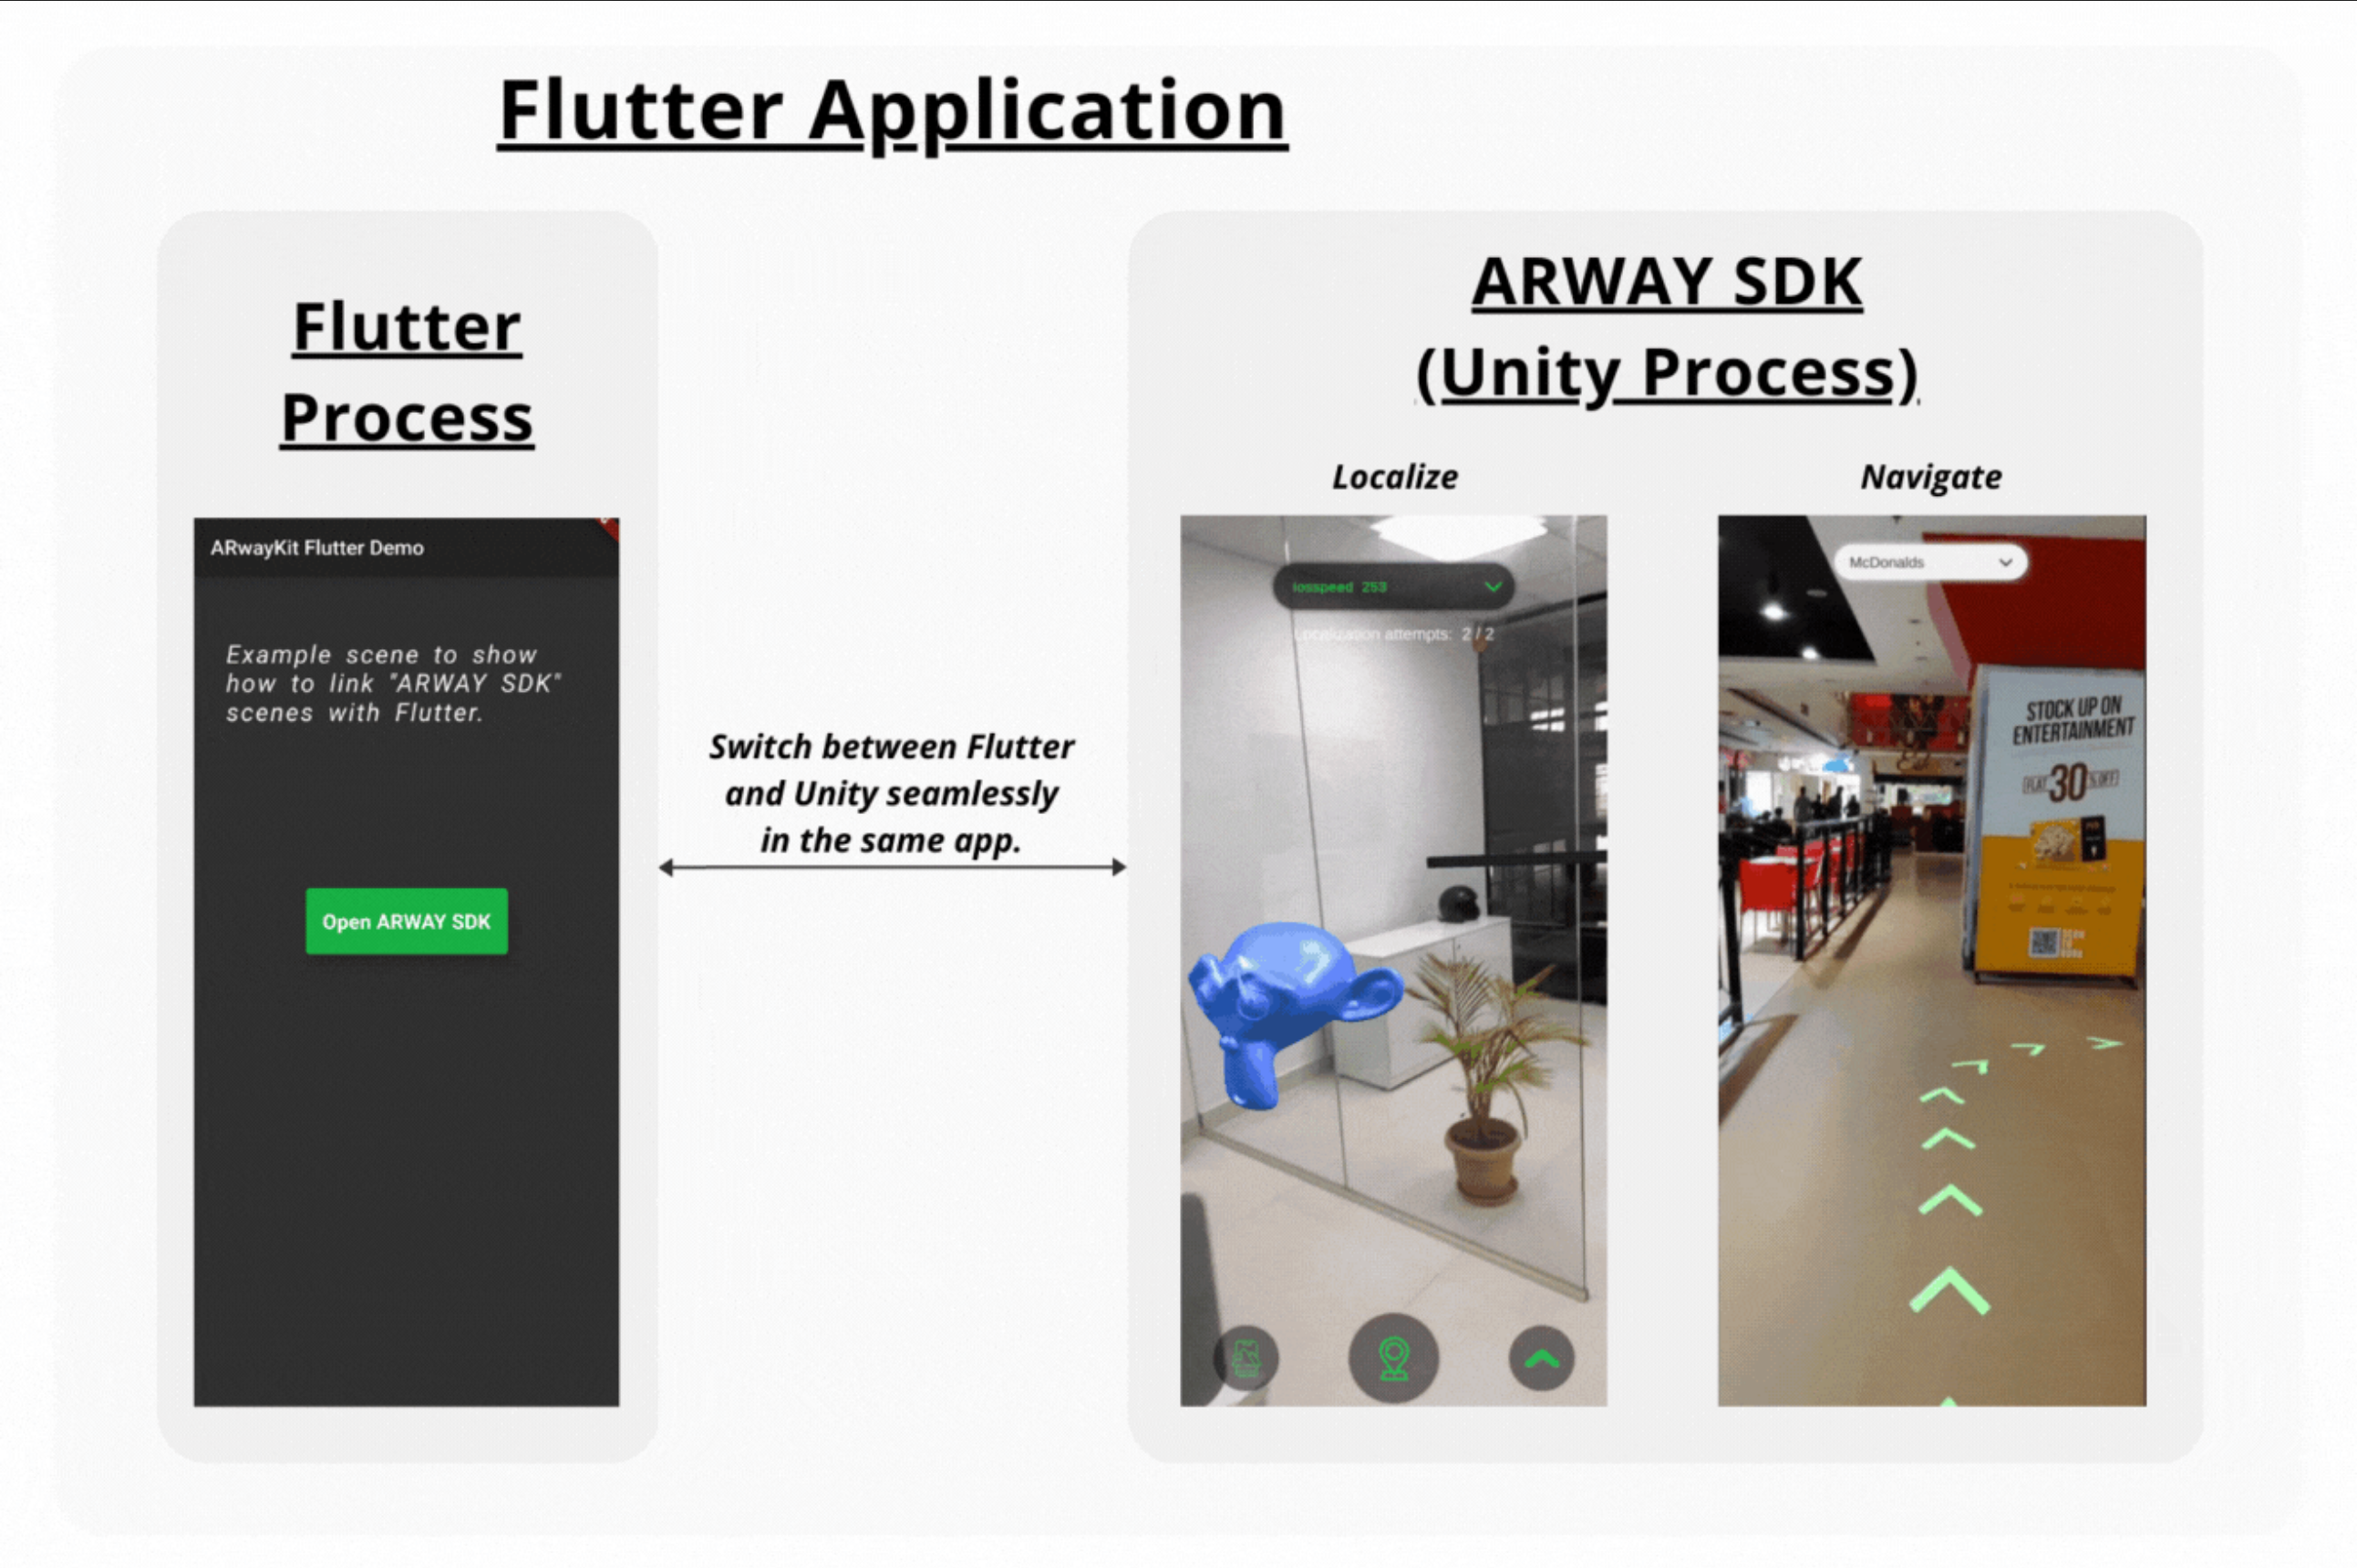
\includegraphics[width=\textwidth]{ARwayKit_samplegif_screenshot}
  \caption[Realtà aumentata con ARwayKit]{Immagine esempio di utilizzo realtà aumentata con ARwayKit\footnotemark}
\end{figure}
\footnotetext{Fonte: \url{https://medium.com/arway/building-ar-navigation-apps-with-flutter-and-arwaykit-280b69401cd9}}

Tuttavia, presenta delle criticità: in primo luogo obbliga l'uso di Unity (sfruttando la sua caratteristica peculiare di poter essere importato come fosse una libreria) per sviluppare la vista in realtà aumentata, il che comporta non solo dover imparare il linguaggio ma dover anche configurare ulteriori componenti (come ad esempio Unity Hub) che poi devono essere adottati assieme a quelli già in uso, appesantendo quindi il processo di codifica.\\
In secondo luogo troviamo invece il problema maggiore: la vista verrebbe realizzata nativamente in Unity, ovvero si tratta di una componente Unity separata rispetto all'applicazione che la lancia.
Questo renderebbe complesso se non impossibile usare dentro essa delle funzionalità Flutter: ad esempio, un bottone a schermo sarebbe un pulsante Unity, non Flutter, obbligando quindi poi a costruire una mappatura tra i due linguaggi per ogni funzionalità visualizzata.\\ 
Una vista così costruita non solo è scomoda da programmare, ma anche difficile da manutenere.

\subsubsection{ar\_flutter\_plugin}
\aplug{} è un \textit{plugin open-source} collaborativo estremamente giovane (il primo \textit{commit} sulla \textit{repository} pubblica risale al 6 febbraio 2021\footnote{Fonte: \url{https://github.com/CariusLars/ar_flutter_plugin/commit/da9ab148219d833755ef7a9b1e3536a3cae865d1}}) che si pone l'obiettivo di implementare componenti in realtà aumentata in Flutter.\\
Per raggiungere lo scopo si serve della libreria archiviata Sceneform\footnote{Fonte: \url{https://developers.google.com/sceneform/develop}}, che si occupa di "renderizzare scene tridimensionali realistiche in applicazioni in realtà aumentata o meno, senza dover imparare OpenGL".\\
L'architettura di \aplug{} è composta da due componenti: una \api{} multipiattaforma unificata che fornisce un'interfaccia alle applicazioni tramite il \textit{plugin} e le implementazioni specifiche per le piattaforme Android (in Kotlin) e iOS (in Swift) costruite su ARCore e ARKit rispettivamente, così da garantire accesso continuativo nel tempo a funzionalità aggiornate.\\
\aplug{} espone dei \textit{widget} che possono essere inclusi nel \textit{widget tree} (fig. \ref{fig:flutter-trees}) dell'applicazione cliente e delle classi \textit{manager} per gestire funzionalità e logiche di controllo del \textit{plugin} e delle componenti in realtà aumentata: il \textit{session manager} gestisce le configurazioni di tracciamento (ad esempio se gestire piani orizzontali, verticali o entrambi), opzioni di \textit{debugging} (come la visualizzazione dei piani) e le \textit{callbacks} per gli \textit{hit-test}\footnote{Immaginando un vettore che parte dall'ottica del dispositivo e tocca una superficie, possiamo considerare quel contatto un \textit{"hit"}. Con \textit{hit-testing} si intende valutare la capacità di tracciare correttamente lo spazio inteso come distanza tra i punti dello stesso e il dispositivo.} e i \textit{gesture events}\footnote{Azioni che il sistema deve fare quando vengono effettuati degli \textit{input} tramite \textit{touch screen} del dispositivo}.\\
L'\textit{object manager} gestisce i nodi in realtà aumentata del \textit{plugin} che servono ad astrarre rispetto alle funzionalità native delle varie piattaforme (ARCore e ARKit ad esempio) e permettono di aggiungere, modificare o rimuovere nodi basandosi su formati GLTF2 o GLB che possono essere caricati a \textit{runtime} da un \textit{file system} o dalla rete.\\
L'\textit{anchor manager} contiene funzioni per caricare e ottenere ancoraggi da servizi \textit{cloud} servendosi della \api{} Google Coud Anchor. Gli ambienti virtuali registrati localmente possono essere salvati in rete e comparati con quelli già in \textit{storage} persistente per scaricare ancoraggi e oggetti precedentemente posizionati nella scena.\\
Infine il \textit{location manager} si occupa di fornire le coordinate del \textit{global positioning system}  per permettere un'interrogazione efficiente degli ancoraggi basati su posizione geografica.\\
Il \textit{plugin} ha un'architettura largamente \textit{clout-agnostic}, ovvero che non si interessa dell'implementazione specifica per i servizi di salvataggio persistente, il che gli permette di usare facilmente gestori di contenuti esterni.

\subsubsection{Confronto}

\subsection{Analisi dei requisiti}
Di seguito sono riportati i requisti individuati nel piano di lavoro proposto e a seguito di opportuni confronti con il tutor aziendale. Essi sono catalogati secondo la dicitura:
\begin{center}
    \textbf{R[Obbligatorietà][Tipologia][Codice]}
\end{center}
dove:
\begin{itemize}
    \item \textbf{Obbligatorietà}: specifica quanto un requisito sia vincolante per la riuscita del prodotto e può assumere i seguenti valori:
    \begin{itemize}
        \item \textbf{1: } Requisito obbligatorio;
        \item \textbf{2: } Requisito desiderabile ma non essenziale per il funzionamento;
        \item \textbf{3: } Requisito opzionale.
    \end{itemize}
    \item \textbf{Tipologia}: specifica la tipologia del requisito e può assumere i seguenti valori:
    \begin{itemize}
        \item \textbf{F: }\textit{funzionale,} determina una funzionalità necessaria all'applicazione;
        \item \textbf{V: }\textit{vincolo,} riguarda una caratteristica del prodotto decisa a monte.
    \end{itemize}
    \item \textbf{Codice}: identifica univocamente un requisito all'interno della sua tipologia (ovvero possono esistere due requisiti con lo stesso codice a patto che siano uno funzionale e uno di vincolo). Per i requisti subordinati si usa il "punto" come divisorio (\textit{ReqPadre, ReqPadre.Figlio1})
\end{itemize}

\subsubsection{Requisiti funzionali}
{
    \setlength{\freewidth}{\dimexpr\textwidth-10\tabcolsep}
    \renewcommand{\arraystretch}{1.5}
    \centering
    \setlength{\aboverulesep}{0pt}
    \setlength{\belowrulesep}{0pt}
    \rowcolors{2}{red!10}{white}
    \begin{longtable}{C{.15\freewidth} | C{1\freewidth}}
       \toprule
    \rowcolor{red}
    \textcolor{white}{\textbf{Codice}}&
    \textcolor{white}{\textbf{Descrizione}}\\
    \toprule
    \endhead

    R1F1 & Il \textit{plugin} deve rappresentare \textit{asset} tramite ancoraggio in realtà aumentata\\
    R1F2 & Il \textit{plugin} deve rappresentare \textit{ticket} tramite ancoraggio in realtà aumentata\\
    R1F3 & Il \textit{plugin} deve integrare gli ancoraggi tramite \asa{}\\
    R1F3.1 & Permettere aggiunta di \asa\\%C
    R1F3.2 & Permettere recupero e visualizzazione di \asa\\%R
    R2F3.3 & Permettere modifica di \asa\\%U
    R1F3.4 & Permettere eliminazione di \asa\\%D
    %API BACKEND
    R1F4 & Comunicare con le \api{}s di Syn\\
    R1F4.1 & Ricevere \textit{asset} con ancoraggio associato\\
    R1F4.2 & Aggiungere \textit{asset} con ancoraggio associato\\
    R2F4.3 & Ricevere \textit{ticket} con ancoraggio associato\\
    R2F4.4 & Aggiungere \textit{ticket} con ancoraggio associato\\
    %UI FLUTTER
    R1F5 & Utente deve poter vedere quali \textit{asset} hanno ancoraggio associato\\
    R2F6 & Utente deve poter vedere quali \textit{ticket} hanno ancoraggio associato\\
    R1F7 & Utente deve poter raggiungere l'ancoraggio in vista in realtà aumentata dalla schermata dell'\textit{asset}\\
    R1F8 & \textit{On-Tap} su una ancoraggio deve aprire una \textit{bottom sheet} contestuale\\
    R1F8.1 & \textit{Bottom sheet} deve presentare identificatore per \textit{asset} o \textit{ticket} associato alla ancoraggio\\
    R1F8.2 & \textit{Bottom sheet} associato a un \textit{asset} mostra ultimi tre \textit{ticket} aperti\\
    R1F8.3 & \textit{Bottom sheet} deve fornire \textit{Call-To-Action} per eliminare l'ancoraggio\\
    R1F8.4 & \textit{Bottom sheet} deve fornire \textit{Call-To-Action} per raggiungere pagina di dettaglio\\
    R1F9 & Le informazioni contestuali di un \textit{ticket} includono data e ora di creazione\\
    %UI AR
    R1F10 & Gli ancoraggi hanno rappresentazione visiva contestuale\\ 
    R1F10.1 & Gli \textit{asset} vengono rappresentati come \todo\\
    R1F10.2 & I \textit{ticket} vengono rappresentati come \todo\\
    R1F11 & \textit{On-Tap} sullo spazio permette di creare una ancoraggio in posizione\\
    R1F11.1 & Ancoraggio posizionato nello spazio può essere salvato\\
    R1F11.2 & Ancoraggio posizionato nello spazio può essere eliminato\\
    R1F12 & Il salvataggio di un'ancoraggio è disponibile solo quando è sicuro vada a buon fine\\
    R1F12.1 & Viene mostrato a schermo un feedback riguardo il livello di sicurezza raggiunto\\
    \bottomrule
    \rowcolor{white} 
    \caption{Tabella dei requisiti funzionali}
    \label{tab:requisiti-funzionali}
    \end{longtable}
}

\subsubsection{Requisiti di vincolo}
{
    \setlength{\freewidth}{\dimexpr\textwidth-10\tabcolsep}
    \renewcommand{\arraystretch}{1.5}
    \centering
    \setlength{\aboverulesep}{0pt}
    \setlength{\belowrulesep}{0pt}
    \rowcolors{2}{red!10}{white}
    \begin{longtable}{C{.15\freewidth} C{1\freewidth}} 
       \toprule
    \rowcolor{red}
    \textcolor{white}{\textbf{Codice}}&
    \textcolor{white}{\textbf{Descrizione}}\\
    \toprule
    \endhead

    R1V1 & \textit{Framework} scelto funziona su Android\\
    R2V2 & \textit{Framework} scelto funziona su iOS\\
    R1V3 & \textit{Framework} scelto si integra con le \api{}s di Syn\\
    R1V3.1 & \textit{Framework} ottiene con ancoraggio associato i dati degli \textit{asset}\\
    R1V3.2 & \textit{Framework} ottiene con ancoraggio associato i dati dei \textit{ticket}\\
    R1V4 & Il \textit{framework} scelto utilizza asa\\
    R1V5 & La vista in realtà aumentata deve essere sviluppata in Flutter\\
    \bottomrule
    \rowcolor{white} 
    \caption{Tabella dei requisiti di vincolo}
    \label{tab:requisiti-di-vincolo}
    \end{longtable}
}

\subsubsection{Riepilogo requisiti}
Sono stati individuati un totale di 36 requisiti, 29 funzionali e 7 di vincolo, di seguito schematizzati:
{
    \setlength{\freewidth}{\dimexpr\textwidth-10\tabcolsep}
    \renewcommand{\arraystretch}{1.5}
    \centering
    \setlength{\aboverulesep}{0pt}
    \setlength{\belowrulesep}{0pt}
    \rowcolors{2}{red!10}{white}
    \begin{longtable}{C{.25\freewidth} C{.2\freewidth}} 
       \toprule
    \rowcolor{red}
    \textcolor{white}{\textbf{Obbligatorietà}}&
    \textcolor{white}{\textbf{Quantità}}\\
    \toprule
    \endhead

    Obbligatori & 31\\
    Desiderabili & 5\\
    \bottomrule
    \rowcolor{white} 
    \caption{Numero di requisiti per obbligatorietà}
    \label{tab:requisiti-obbligatorieta}
    \end{longtable}
}

{
    \setlength{\freewidth}{\dimexpr\textwidth-10\tabcolsep}
    \renewcommand{\arraystretch}{1.5}
    \centering
    \setlength{\aboverulesep}{0pt}
    \setlength{\belowrulesep}{0pt}
    \rowcolors{2}{red!10}{white}
    \begin{longtable}{C{.25\freewidth} C{.2\freewidth}} 
       \toprule
    \rowcolor{red}
    \textcolor{white}{\textbf{Tipologia}}&
    \textcolor{white}{\textbf{Quantità}}\\
    \toprule
    \endhead

    Funzionali & 29\\
    Di Vincolo & 7\\
    \bottomrule
    \rowcolor{white} 
    \caption{Numero di requisiti per tipologia}
    \label{tab:requisiti-tipolgia}
    \end{longtable}
}

\subsection{Attività di supporto}
\subsubsection{Interazione aziendale}
\subsubsection{Processi di verifica e validazione}
%************************************************************************************************************
\section{Difficoltà incontrate}
\subsection{Problemi documentali}
\subsection{Problemi tecnologici}

%************************************************************************************************************

\section{Risultati raggiunti}
\subsection{Copertura requisiti}
\subsection{Implementazione Android}
\subsection{Implementazione iOS}

% !TEX encoding = UTF-8
% !TEX TS-program = pdflatex
% !TEX root = ../tesi.tex

%**************************************************************
\chapter{Valutazione Retrospettiva}
\label{cap:valutazione-retrospettiva}
%**************************************************************

\section{Soddisfacimento obiettivi}
\subsection{Valutazione personale}
\subsection{Valutazione proponente}

\section{Competenze}
\subsection{Competenze acquisite}
\subsection{Competenze mancanti}
\subsubsection{Lacune corso di studi}

\begin{appendices}
    
\chapter{Flutter}
\label{ch:flutter}
E' impossibile parlare di Flutter senza prima discutere del linguaggio su cui si basa: Dart.\\
Faremo quindi un'introduzione quanto più sintetica possibile sulle sue caratteristiche più proprietarie, tralasciando invece le similitudini a linguaggi popolari che possono facilmente essere intuite dal lettore.
\section{Dart}
Dart è un linguaggio compilato fortemente tipizzato con sintassi simile a C, e adotta molte funzionalità tipiche dei linguaggi moderni: considera infatti ogni variabile un oggetto e implementa la \textit{null safety}, obbligando il programmatore a esplicitare con sintassi specifiche la presenza o meno del valore \verb+null+.

\begin{lstlisting}[language=dart, firstnumber=1,caption={Dart \textit{null safety}}]
//dichiarazione di variabili
String variabileNotNullable = '';  //non puo' mai essere null
String? variabileNullable = null;  //puo' anche essere null

//utilizzo esplicito di variabile nullable
fun (variableNullable);   //compile error
fun (?variableNullable);  //esplicito che puo' essere nulla

//utilizzo esplicito di variabile not nullable
if (value != null)
    fun (!value);   //dico al compilatore che sono certo value != null
\end{lstlisting} 

Permette inoltre l'interpolazione di stringhe:

\begin{lstlisting}[language=dart, firstnumber=1,caption={Dart interpolazone stringhe}]
//sfrutto il simbolo $
'number = $variableName';              //inserisco in stringa 
                                       //direttamente una variabile
'expressionResult = ${expression}';    //inserisco in stringa
                                       //direttamente un'espressione
\end{lstlisting}

Dart tratta in maniera particolare le funzioni, che sono oggetti, hanno un tipo (\verb+Function+), possono avere parametri posizioni o nominali, obbligatori od opzionali: 

\begin{lstlisting}[language=dart, firstnumber=1,caption={Dart parametri funzioni}]
//parametri obbligatori posizionali
void fun (int a, int b);  //non possono essere nulli

//possono essere anteceduti da parametri posizionali opzionali
void fun (int a, int b, [String opz1 = '', String opz2 = '']){}
void fun (int a, int b, [String? opz1nullable, String? opz2nullable]){}

//oppure possono essere anteceduti da parametri nominali opzionali
void fun (int a, int b, {String opz1 = '', String opz2 = ''}){}
void fun (int a, int b, {String? opz1nullable, String? opz2nullable}){}

//non possono essere anteceduti da entrambi
//il seguente codice non compila:
void fun (int a, int b, [String opz1 = ''], {String opz2 = ''}){} 

//tutti i costruttori in Dart hanno solo parametri nominali
//di default i parametri nominali sono opzionali
//possono pero' essere resi obbligatori con la keyword 'required'
void fun ({required String obb1, 
           required String? obb2, 
           String opz1 = ''}){}
\end{lstlisting}

Esistono le funzioni anonime (largamente sfruttate nei metodi \verb+build+ di Flutter), che possono essere ovviamente passate come argomento ad altre funzioni, essendo oggetti:

\begin{lstlisting}[language=dart, firstnumber=1,caption={Dart funzioni anonime}]
//prima sintassi
(){
    //corpo della funzione anonima
} 

//seconda sintassi
() => return_expression

//assegnamento di funzione anonima ad una variabile
//ritorna una stringa con un messaggio portato in upper case
var upperfy = (msg) => '${msg.toUpperCase()}';

//passaggio di funzione come parametro
fun (firstValue, () => secondValue);
\end{lstlisting}

Abbiamo delle espressioni condizionali specifiche del linguaggio dalla grande espressività e che quindi vengono largamente usate:

\begin{lstlisting}[language=dart, firstnumber=1,caption={Dart espressioni ternarie}]
//primo tipo di condizione, detta ternaria
condizione ? expr1 : expr2;

//equivale a (in pseudocodice):
if (condizione == true) return expr1
else                    return expr2

//vediamo un esempio
int? a;               //a==null di default
a = a==null ? 1 : 0;  //ad 'a' viene assegnato il valore 1 
                      //siccome a==null


//################################
//secondo tipo di condizione peculiare:
expr1 ?? expr2;

//equivale a (in pseudocodice):
if (expr1 != null) return expr1
else               return expr2

//vediamo un esempio
int? a;      //a==null di default
a = a ?? 1;  //ad 'a' viene assegnato il valore 1 siccome a==null
\end{lstlisting}

I caratteri \verb+?+ e \verb+!+ sono, come si evince dalle espressioni ternarie e dalla \textit{null safety}, di cruciale importanza in Dart, ed è quindi opportuno vederne ancora qualche esempio:

\begin{lstlisting}[language=dart, firstnumber=1,caption={Dart operatori '?' e '!'}]
list[1]     //accede al secondo elemento della lista

list.?[1]
//equivale a (in pseudocodice):
if (list[1] != null)    return list[1]
else                    return null

//##############################

foo?.bar 
//equivale a (in pseudocodice):
if (foo.bar != null)    return foo.bar
else                    return null

//##############################

foo!.bar
//equivale a (in pseudocodice):
if (foo.bar != null)    return foo.bar
else                    throw (runtimeException)
\end{lstlisting}

Le applicazioni \textit{mobile} e \textit{web} spesso si trovano a eseguire istruzioni che richiedono l'attesa di risorse esterne (ottenere dati dalla rete o leggerli da un \textit{file}, oppure scrivere su un \textit{database}). Per evitare il completo blocco dell'esecuzione (disastroso per un applicativo \textit{consumer}) Dart implementa nativamente delle funzioni di programmazione asincrona, che permetto di svolgere operazioni anche mentre altre sono in attesa.\\
Per fare ciò si serve di tre \textit{keyword}: \verb+async+, \verb+await+ e \verb+Future+:

\begin{lstlisting}[language=dart, firstnumber=1,caption={Dart programmazione asincrona}]
Future<void> checkVersion () async {
    var version = await lookUpVersion();
}

//un'espressione marcata con la keyword 'await' ritorna sempre Future<T>
\end{lstlisting}

Trattiamo infine le caratteristiche peculiari di Dart per quanto riguarda classi e metodi:

\begin{itemize}
    \item Esistono i costruttori costanti, marcati \verb+const+, che sono inizializzati a \textit{compile-time}. Tutti gli altri sono implicitamente dinamici (quindi \textit{run-time});
    \item Posso creare costruttori nominati per implementare costruttori multipli tramite la sintassi:
\begin{lstlisting}[language=dart]
ClassName.constructorName () :
    firstField = firstValue,
    secondField = secondValue;
\end{lstlisting}
    \item Ogni entità è una classe, ogni classe discende da \verb+Object+ (a eccezione di \verb+Null+);
    \item Per ogni classe viene creata un'interfaccia implicita che contiene tutti i membri d' istanza della classe;
    \item I metodi \textit{getter} e \textit{setter} di una classe vengono creati implicitamente per variabili non \verb+final+, ma possono essere definiti esplicitamente con le \textit{keyword} \verb+get+ e \verb+set+.
\end{itemize}

\section{Widget}
Mostriamo ora alcuni componenti di Flutter necessari al proseguimento della lettura, partendo dai \textit{widget}: riprendono l'idea di React di costruire tutta l'interfaccia grafica tramite uno \textit{stack} di \textit{widget}, che definiscono il proprio aspetto basandosi sulla configurazione e lo stato attuali. Quando lo stato di un \textit{widget} cambia, esso riscrive la propria descrizione (insieme di istruzioni e valori che lo determinano) e il \textit{framework} valuta le differenze tra questa e la descrizione precedente per apportare le modifiche necessarie al suo \textit{render tree} e quindi, ultimamente, modificarne l'aspetto e finalizzare il cambio di stato.

\begin{figure}[H]
    \centering
    \includegraphics[width=\textwidth]{Flutter_trees}
    \caption[I tre alberi di Flutter]{Flutter usa tre alberi logici come rappresentazione delle proprie strutture: uno per i \textit{widget}, uno per gli \textit{element} e infine quello di \textit{render}.\footnotemark}
    \label{fig:flutter-trees}
\end{figure}
\footnotetext{Fonte: \url{https://docs.flutter.dev/resources/architectural-overview}}

L'albero di \textit{render} è una delle tre strutture logiche che Flutter usa per descrivere i propri oggetti e le proprie interfacce grafiche: \textit{widget tree}, \textit{element tree} e \textit{render tree}. \\
Il \textit{widget tree} rappresenta gli elementi di un \textit{widget} come uno \textit{stack} di \textit{widget}, messi in relazione con il loro elemento padre e i loro elementi figli. Quello mostrato in figura \ref{fig:flutter-trees}, ad esempio, rappresenta un \verb+Containter+ che contiene un \verb+ColoredBox+ che a sua volta contiene una \verb+Row+ e via dicendo. I \textit{widget} sono per definizione immutabili, quindi una modifica richiede necessariamente una distruzione e successiva ricreazione del \textit{widget} interessato.\\
Vediamo un esempio più specifico di \textit{widget tree}:

\begin{lstlisting}[language=dart, caption={Codice rilevante per la parte grafica dell'\textit{app} di esempio di Flutter}]
Widget build(BuildContext context) {
    return Scaffold(
      appBar: AppBar(
        title: Text(widget.title),
      ),
      body: Center(
        child: Column(
          mainAxisAlignment: MainAxisAlignment.center,
          children: <Widget>[
            const Text(
              'You have pushed the button this many times:',
            ),
            Text(
              '$_counter',
              style: Theme.of(context).textTheme.headline4,
            ),
          ],
        ),
      ),
      floatingActionButton: FloatingActionButton(
        onPressed: _incrementCounter,
        tooltip: 'Increment',
        child: const Icon(Icons.add),
      ), 
    );
}
\end{lstlisting}

Il codice precedente produce il seguente risultato (e il seguente \textit{widget tree}):

\begin{figure}[H]
    \centering
    \includegraphics[height=8cm]{app_esempio_render_tree.png}\hspace{15mm}
    \includegraphics[height=8cm]{flutter_app_default.jpg}
    \caption[\textit{Widget tree} app esempio]{Il \textit{widget tree} dell'applicazione di esempio di Flutter e il suo risultato su Android}
\end{figure}

Per quanto riguarda le dimensioni delle varie componenti, Flutter ragiona come segue: i padri passano ai figli (dall'altro verso il basso nel \textit{widget tree}) dei \textit{"constraints"}, ovvero le dimensioni massime oltre le quali non possono cresce, e i figli passano quindi ai padri (dal basso verso l'alto nel \textit{widget tree}) le proprie dimensioni.\\
Il \textit{widget tree} è quello più importante da tenere a mente, e che più direttamente si interfaccia con il codice scritto dal programmatore. \\
Torniamo però alla figura \ref{fig:flutter-trees} per parlare brevemente degli altri due alberi: l'\textit{element tree} rappresenta gli elementi che, a differenza dei \textit{widget}, sono mutabili e vengono definiti come "un'istanza di un \textit{widget} in una particolare posizione dell'albero". Gli elementi sono responsabili di aggiornare l'interfaccia utente e fungono da ponte tra \verb+Widget+ e \verb+Render Object+.\\
Il \textit{render tree} rappresenta i \verb+Render Object+ e viene interpellato dal \textit{framework} per disegnare i componenti dell'interfaccia grafica. Una singola istanza di \verb+Render Object+ contiene tutte le informazioni riguardanti dimensioni, colori e logiche di \textit{layout} di un \verb+Widget+.\\
Abbiamo accennato che i \textit{widget} quando cambiano stato richiamano il proprio metodo \verb+build+ che provoca quindi una ricostruzione del \textit{widget} stesso. Questi \textit{widget} si chiamano "\textit{stateful}", e sono in diretta contrapposizione con quelli incapaci di modificarsi durante l'esecuzione, chiamati "\textit{stateless}". \\
Vediamo un esempio di \textit{stateful widget}:

\begin{lstlisting}[language=dart, label={lst:stateful_widget}, caption={Creazione \textit{stateless widget}}]
class MyApp extends StatelessWidget {
  //stateless widget che fa da radice per l'applicazione
  const MyApp({super.key});

  @override
  Widget build(BuildContext context) {
    return MaterialApp(
        home: const MyHomePage(title: 'Flutter Demo Home Page'),
    );
  }
}

class MyHomePage extends StatefulWidget {
  //qui passiamo allo stateful widget
  const MyHomePage({super.key, required this.title});
  final String title;

  @override
  //e qui creiamo lo stato vero e proprio
  State<MyHomePage> createState() => _MyHomePageState();
}


class _MyHomePageState extends State<MyHomePage> {
  int _counter = 0;

  void _incrementCounter() {
    //quando viene chiamata questa funzione viene
    //richiamato il metodo build, di fatto cambiando lo stato 
    //del widget e provocando un re-render dell'applicazione
    setState(() {
      _counter++;
    });
  }

  @override
  Widget build(BuildContext context) {}
}
\end{lstlisting}

Si nota immediatamente che l'uso degli \textit{stateful widget} provoca scrittura di codice ridondante e si è quindi deciso di arginare questo problema, aumentando al contempo la condivisione di codice tra i \textit{widget}, introducendo i Flutter Hooks (ispirati dagli \textit{hooks} di React).
Vediamo quindi la riscrittura del codice mostrato nel frammento \ref{lst:stateful_widget} opportunamente modificato usando un \verb+HookWidget+:

\begin{lstlisting}[language=dart, caption={Creazione \textit{hook widget}}]
class MyApp extends StatelessWidget {
  //stateless widget che fa da radice per l'applicazione
  const MyApp({super.key});

  @override
  Widget build(BuildContext context) {
    return MaterialApp(
        home: const MyHomePage(title: 'Flutter Demo Home Page'),
    );
  }
}

class MyHomePage extends HookWidget {
  //basta questa classe per fare tutti gli step
  //necessari al cambio di stato

  const MyHomePage({super.key, required this.title});
  final String title;

  Widget  build (BuildContext context){
    //_counter viene inizializzato a zero e reso
    //l'hook per il cambio di stato, quindi quando
    //il suo valore cambia viene provocato un rebuild
    final _counter = useState(0)

    return Scaffold(
      appBar: AppBar(),
      body: Center(),
      floatingActionButton: FloatingActionButton(
        //qui il valore di _counter cambia
        //provocando una rebuild
        onPressed: () => _counter.value++,
      )
    )
  }
}
\end{lstlisting}

\section{Method Channels}
I \textit{method channel} nascono per uno scopo: utilizzare codice nativo tramite Flutter, ad esempio per chiamare \api{} \textit{platform-specific} in Kotlin o Java per Android, in Swift per iOS o in C++ per Windows.\\
Flutter non usa queste funzionalità tramite generazione di codice e preferisce un approccio basato sullo scambio di messaggi. Vediamone quindi un esempio per ottenere, tramite Java, il valore di carica della batteria di un dispositivo Android.\\
Per prima cosa è necessario agire sull'Android \textit{manifest} inserendo il nome dell'applicazione di Flutter, in questo caso \verb+batterylevel+ (l'applicazione si può creare con il comando: \verb+flutter create nome_applicazione+).

\begin{lstlisting}[language=XML, firstnumber=1,caption={Android \textit{manifest}}]
<manifest xmlns:android="http://schemas.android.com/apk/res/android"
  package="com.example.batterylevel">
\end{lstlisting}

A questo punto si vanno a costruire gli "agganci" per il \textit{method channel} in codice nativo, in questo caso quindi nell'attività principale di Java:

\begin{lstlisting}[language=Java, firstnumber=1,caption={Java \textit{main activity}}]
public class MainActivity extends FlutterActivity {
  //"samples.flutter.dev/battery" e' il nome del method channel
  //come definito in main.dart
  private static final String CHANNEL = "samples.flutter.dev/battery";

  @Override
  public void configureFlutterEngine(@NonNull FlutterEngine flutterEngine) {
      super.configureFlutterEngine(flutterEngine);
      new MethodChannel(flutterEngine.getDartExecutor()
                                     .getBinaryMessenger(), CHANNEL)
              .setMethodCallHandler(
                      (call, result) -> {
                          //Questo e' il metodo invocato nel main
                          //sfruttiamo "getBatteryLevel" per invocarlo
                          if (call.method.equals("getBatteryLevel")) {
                              //il metodo vero e proprio in Java
                              int batteryLevel = getBatteryLevel();
                              if (batteryLevel != -1) {
                                  result.success(batteryLevel);
                              } else {
                                  result.error("UNAVAILABLE", 
                                  "Battery level not available.", null);
                              }
                          } else {
                              result.notImplemented();
                          }
                      }
              );
  }

  private int getBatteryLevel() {
    //metodo che ritorna il valore di batteria del dispositivo
  }
\end{lstlisting}

Infine ci occupiamo di lanciare il messaggio da Flutter invocando il metodo:

\begin{lstlisting}[language=dart, firstnumber=1,caption={Dart \textit{main}}]
class MyHomePage extends HookWidget {
const MyHomePage({super.key});
//creo e definisco il method channel
static const platform = MethodChannel('samples.flutter.dev/battery');

  @override
  Widget build(BuildContext context) {
    var batteryLevel = useState('Unknown battery level.');

    return Material(
      child: Center(
        child: Column(
          mainAxisAlignment: MainAxisAlignment.spaceEvenly,
          children: [
            ElevatedButton(
              onPressed: () async {
                try {
                  //qui avviene l'effettiva invocazione del
                  // method channel che provoca una chiamata in Java
                  final int result =
                      await platform.invokeMethod('getBatteryLevel');
                  batteryLevel.value = 'Battery level at $result % .';
                } on PlatformException catch (e) {
                  batteryLevel.value =
                      "Failed to get battery level: '${e.message}'.";
                }
              },
              child: const Text('Get Battery Level'),
            ),
            Text(batteryLevel.value),
          ],
        ),
      ),
    );
  }
}
\end{lstlisting}

\end{appendices}

%**************************************************************
% Materiale finale
%**************************************************************
\backmatter
%\printglossaries
\printglossary[type=\acronymtype, title=Acronimi e abbreviazioni, toctitle=Acronimi e abbreviazioni]
\printglossary[type=main, title=Glossario, toctitle=Glossario]
\input{inizio-fine/bibliografia}
\end{document}
